        %%******************************************%%
        %%                                          %%
        %%        Modello di tesi di laurea         %%
        %%            di Andrea Giraldin            %%
        %%                                          %%
        %%             2 novembre 2012              %%
        %%                                          %%
        %%******************************************%%

\begin{document}
    \frontmatter
    \begin{titlepage}
    \begin{center}
        \begin{LARGE}
            \textbf{\myUni}\\
        \end{LARGE}

        \vspace{10pt}

        \begin{Large}
            \textsc{\myDepartment}\\
        \end{Large}

        \vspace{10pt}

        \begin{large}
            \textsc{\myFaculty}\\
        \end{large}

        \vspace{30pt}
        \begin{figure}[htbp]
            \centering
            
\includegraphics[height=6cm]{unipd-logo}
        \end{figure}
        \vspace{30pt}

        \begin{LARGE}
            \textbf{\myTitle}\\
        \end{LARGE}

        \vspace{10pt}

        \begin{large}
            \textsl{\myDegree}\\
        \end{large}

        \vspace{40pt}

        \begin{large}
            \begin{flushleft}
                \textit{Relatore}\\
                \vspace{5pt}
                \profTitle\ \myProf
            \end{flushleft}

            % You can tweak the spacing to have professor and student names on the same line
            % useful if the page is broken by a long thesis title and you need more space
            % \vspace{-52pt}

            \begin{flushright}
                \textit{Laureando}\\
                \vspace{5pt}
                \myName \\
                \vspace{5pt}
                \textit{Matricola} \myID
            \end{flushright}
        \end{large}

        \vspace{40pt}

        \line(1, 0){338} \\
        \begin{normalsize}
            \textsc{Anno Accademico \myAA}
        \end{normalsize}
    \end{center}
\end{titlepage}

    \clearpage
\phantomsection
\thispagestyle{empty}

\hfill
\vfill

\noindent\myName: \textit{\myTitle,}
\myDegree,
\textcopyright\ \myTime.

    % \cleardoublepage
\phantomsection
\thispagestyle{empty}
\pdfbookmark{Dedica}{Dedica}

\vspace*{3cm}

\begin{center}
    Lorem ipsum dolor sit amet, consectetuer adipiscing elit. \\ \medskip
    --- Oscar Wilde
\end{center}

\medskip

\begin{center}
    Dedicato a ...
\end{center}
 % Non ho una persona speciale a cui dedicare la tesi
    \cleardoublepage
\phantomsection
\pdfbookmark{Ringraziamenti}{ringraziamenti}

\begin{flushright}{
    \slshape
    ``La differenza tra una persona di successo e gli altri non è la mancanza di forza, né la mancanza di conoscenza, ma piuttosto la mancanza di volontà.''} \\
    \medskip
    --- Vince Lombardi
\end{flushright}


\bigskip

\begingroup
\let\clearpage\relax
\let\cleardoublepage\relax
\let\cleardoublepage\relax

\chapter*{Ringraziamenti}

\noindent \textit{Innanzitutto, vorrei esprimere la mia gratitudine al Prof. \myProf, relatore della mia tesi, per l'aiuto e il sostegno fornitomi durante la stesura del lavoro.}\\

\noindent \textit{Desidero ringraziare con affetto i miei genitori per il sostegno, il grande aiuto e per essermi stati vicini in ogni momento durante gli anni di studio.}\\

\noindent \textit{Ho desiderio di ringraziare poi i miei amici per tutti i bellissimi anni passati insieme e le mille avventure vissute.}\\
\bigskip

\noindent\textit{\myLocation, \myTime}
\hfill \myName

\endgroup

    \cleardoublepage
\phantomsection
\pdfbookmark{Sommario}{Sommario}
\begingroup
\let\clearpage\relax
\let\cleardoublepage\relax
\let\cleardoublepage\relax

\chapter*{Sommario}

Questo elaborato descrive l’attività svolta da Stefani Riccardo durante un tirocinio curriculare della durata di 320 ore presso l’azienda Oribea AI S.r.l.

Il progetto si inserisce negli ambiti della Business Intelligence e del Machine Learning, con l'obiettivo di sviluppare una Task AI per l'analisi delle vendite, utilizzando dati provenienti da database aziendali o dataset pubblici. Il sistema realizzato sfrutta un Large Language Model (LLM) per generare analisi automatiche, interpretabili e personalizzabili.

Inoltre, il progetto prevede anche lo sviluppo di un sistema di raccomandazione integrato in un'apposita Task AI, che permetta di raccomandare prodotti ai clienti in base alle loro preferenze e comportamenti di acquisto, e viceversa di suggerire possibili clienti a cui proporre i prodotti, ottimizzando le strategie di marketing e vendita.

Prima della fase di sviluppo, è stato condotto uno studio approfondito delle tecnologie impiegate e dei concetti economici fondamentali per garantire la qualità delle analisi delle vendite e delle raccomandazioni prodotte. Le attività e le soluzioni adottate vengono illustrate nei capitoli successivi.

%\vfill

%\selectlanguage{english}
%\pdfbookmark{Abstract}{Abstract}
%\chapter*{Abstract}

%\selectlanguage{italian}

\endgroup

\vfill

    \cleardoublepage
\pdfbookmark{\contentsname}{tableofcontents}
\setcounter{tocdepth}{2}
\tableofcontents
%\markboth{\contentsname}{\contentsname}
\clearpage

\begingroup
    \let\clearpage\relax
    \let\cleardoublepage\relax
    \let\cleardoublepage\relax

    % Figures list
    \phantomsection
    \pdfbookmark{\listfigurename}{lof}
    \listoffigures

    \vspace*{8ex}

    % Tables list
    \phantomsection
    \pdfbookmark{\listtablename}{lot}
    \listoftables

    \vspace*{8ex}
\endgroup

\cleardoublepage

    \cleardoublepage

    \mainmatter
    \chapter{Introduzione}
\label{cap:introduzione}

\intro{In questo capitolo verrà descritta l’azienda proponente del tirocinio, il way of working, l’organizzazione del testo e delle convenzioni tipografiche impostate.}\\

\section{L'azienda}

Oribea AI S.r.l. è una startup innovativa fondata nel 2024 nella Repubblica di San Marino, in seguito alla separazione dall'azienda di e-commerce ITTweb. La missione di Oribea è fornire soluzioni avanzate di intelligenza artificiale per migliorare l'efficienza e la produttività delle aziende, con un focus particolare sull'implementazione di \gls{llm} e agenti intelligenti.
Tra i principali prodotti sviluppati da Oribea vi è l'AI Agent Builder, uno strumento che consente alle imprese di creare e integrare agenti intelligenti personalizzati nei propri processi aziendali. Questi agenti sono progettati per automatizzare attività ripetitive, migliorare la comunicazione interna ed esterna e supportare la presa di decisioni attraverso l'analisi avanzata dei dati. L'AI Agent Builder si distingue per la sua capacità di adattarsi alle specifiche esigenze di ciascuna azienda, offrendo soluzioni su misura che sfruttano le potenzialità degli LLM.
Inoltre, Oribea sta sviluppando un Sistema Intelligente, concepito per fungere da piattaforma centrale nell'orchestrazione delle attività aziendali. Questo sistema mira a integrare diverse applicazioni e servizi, facilitando la gestione dei processi e migliorando la coerenza e l'efficienza operativa. Attraverso l'uso di tecnologie avanzate di intelligenza artificiale, il Sistema Intelligente di Oribea promette di trasformare il modo in cui le aziende operano, rendendo i processi più fluidi e reattivi alle esigenze del mercato.
La scelta di stabilire la sede a San Marino non è casuale: la Repubblica si sta posizionando come un hub per l'innovazione tecnologica, offrendo un ambiente favorevole allo sviluppo e alla sperimentazione di nuove tecnologie. In questo contesto, Oribea beneficia di un ecosistema dinamico e di una rete di collaborazioni che favoriscono la crescita e l'innovazione.
In sintesi, l'aziemda rappresenta un esempio di come le startup possano contribuire significativamente all'evoluzione del panorama tecnologico, offrendo soluzioni innovative che rispondono alle sfide contemporanee delle aziende. La sua focalizzazione sull'intelligenza artificiale applicata ai processi aziendali la rende un attore rilevante nel contesto della trasformazione digitale.

\begin{figure}
    \centering
    
\includegraphics[width=0.5\textwidth]{logo/oribea-logo.png}
    \caption{Logo di Oribea AI S.r.l.}
    \label{fig:oribea-logo}
\end{figure}

\section{L'idea}

L'idea dello stage è nata dalla necessità di sviluppare un sistema che consenta di generare automaticamente un report di analisi delle vendite per un'azienda di e-commerce. Questo report deve essere generato in modo autonomo, senza la necessità di intervento umano, e deve essere in grado di analizzare i dati delle vendite, identificare tendenze e fornire raccomandazioni per migliorare le performance aziendali.

In aggiunta, dallo stesso dataset delle vendite, il sistema deve essere in grado di generare un sistema di raccomandazioni per i clienti, suggerendo prodotti in base alle loro preferenze e comportamenti di acquisto. Questo approccio mira a migliorare l'esperienza del cliente e aumentare le vendite attraverso raccomandazioni personalizzate. Il sistema deve anche suggerire possibili clienti a cui proporre i prodotti, in modo da ottimizzare le strategie di marketing e vendita.
L'obiettivo finale è quello di creare un sistema integrato che possa automatizzare e ottimizzare i processi di analisi delle vendite e raccomandazione dei prodotti, contribuendo così a migliorare l'efficienza operativa dell'azienda e a massimizzare le opportunità di vendita.

Ho scelto questo progetto di stage con il desiderio di approfondire le mie conoscenze nel campo dell'intelligenza artificiale e del machine learning, gli argomenti di cui sono più interessato, in particolare nell'ambito dell'analisi dei dati e delle raccomandazioni personalizzate.

\section{Organizzazione del testo}

\subsection{Struttura del documento}
\label{sec:organizzazione-testo}
Il presente documento è suddiviso in otto capitoli il cui contenuto è brevemente riassunto in seguito:

\begin{description}
    \item[{\hyperref[cap:descrizione-stage]{Il secondo capitolo}}] descrive nel dettaglio il progetto di stage, le tecnologie utilizzate e il modo di lavorare dell'azienda; inoltre, viene fornita un'analisi dei rischi e delle soluzioni adottate per affrontarli;
    
    \item[{\hyperref[cap:analisi-requisiti]{Il terzo capitolo}}] approfondisce l'analisi dei requisiti del sistema, con particolare attenzione alla definizione dei casi d'uso e dei requisiti funzionali e non funzionali, con apposito tracciamento;
    
    \item[{\hyperref[cap:report-vendite]{Il quarto capitolo}}] approfondisce la teoria che sta ala base del report di analisi delle vendite, con particolare attenzione allo studio dei dati, delle tecniche di analisi utilizzate e dei grafici generati;
    
    \item[{\hyperref[cap:sistema-raccomandazione]{Il quinto capitolo}}] approfondisce la teoria che sta alla base del sistema di raccomandazione, con particolare attenzione allo studio di sistemi reali e delle tecniche di raccomandazione e valutazione dei risultati utilizzate;
    
    \item[{\hyperref[cap:progettazione-implementazione]{Il sesto capitolo}}] approfondisce la progettazione e l'implementazione del sistema, con particolare attenzione alla scelta delle tecnologie utilizzate e al loro utilizzo;
    
    \item[{\hyperref[cap:verifica-validazione]{Il settimo capitolo}}] approfondisce le attività di verifica e validazione del sistema, con particolare attenzione ai test di unità sviluppati e all'approccio adottato per i test riguardanti l'LLM;
    
    \item[{\hyperref[cap:conclusioni]{L'ottavo capitolo}}] rappresenta una sintesi finale del lavoro svolto durante il periodo di tirocinio, descrivendo eventuali successi e difficoltà incontrate durante il percorso. Vengono inoltre analizzati i risultati ottenuti rispetto agli obiettivi iniziali così come l’insieme di competenze teoriche e pratiche acquisite nel corso del progetto. Il documento si conclude con una riflessione critica sull’operato e sulla crescita personale e professionale del laureando Riccardo Stefani durante il tirocinio. Infine, viene fornita una panoramica delle prospettive future per il progetto e per l'azienda, evidenziando le opportunità di sviluppo e miglioramento.

\end{description}

\subsection{Convenzioni tipografiche}
\label{sec:convenzioni-tipografiche}

In merito alla redazione del presente documento, sono state adottate le seguenti convenzioni tipografiche:
\begin{itemize}
	\item Gli acronimi, le abbreviazioni e i termini ambigui o di uso non comune menzionati vengono definiti nel glossario, situato alla fine del presente documento;

	\item Per la prima occorrenza in ogni capitolo dei termini riportati nel glossario viene utilizzato il seguente stile: \gls{api};

	\item I termini particolarmente rilevanti in una sezione e quelli in lingua straniera non di uso comune o facenti parti del gergo tecnico sono evidenziati con il carattere \emph{corsivo}, fatta eccezione per le occorrenze presenti nei titoli delle sezioni o nelle didascalie;

	\item I comandi di terminale, i frammenti di codice sorgente e i nomi di file o directory sono evidenziati con il carattere \texttt{monospaziato}.

\end{itemize}

    %\chapter{Processi e metodologie}
\label{cap:processi-metodologie}

\intro{Brevissima introduzione al capitolo}\\

\section{Processo sviluppo prodotto}
 % Processi e metodologie, non consigliato da Zanella. Io lo scriverò nella progettazione
    \chapter{Descrizione dello stage}
\label{cap:descrizione-stage}

\intro{In questa sezione viene presentata una descrizione dell’idea e delle tecnologie utilizzate durante il percorso di stage, e una panoramica del modo di lavorare dell'azienda. Viene inoltre presentata un'analisi dei rischi e delle problematiche riscontrate durante lo sviluppo del progetto.}\\

\section{Introduzione al progetto}

Nel contesto attuale, i report delle vendite e i sistemi di raccomandazione rivestono un ruolo fondamentale per le aziende che operano in mercati competitivi e digitalizzati. I report delle vendite consentono di monitorare l’andamento commerciale, identificare trend, valutare le performance dei prodotti e prendere decisioni strategiche basate su dati concreti. Questi strumenti permettono di individuare rapidamente eventuali criticità o opportunità di crescita, ottimizzando così le strategie di vendita e marketing.\\

Parallelamente, i sistemi di raccomandazione sono diventati essenziali per migliorare l’esperienza utente e incrementare le vendite, soprattutto nelle piattaforme di e-commerce e nei servizi digitali. Attraverso l’analisi dei dati di acquisto e delle preferenze degli utenti, questi sistemi suggeriscono prodotti o servizi personalizzati, aumentando la probabilità di acquisto e la fidelizzazione del cliente. L’integrazione di report delle vendite e sistemi di raccomandazione consente quindi alle aziende di offrire un servizio più mirato ed efficiente, rafforzando la propria posizione sul mercato.\\

In questo contesto, la startup Oribea, che propone soluzioni digitali intelligenti per le aziende, ha ricevuto una commissione da parte di un'azienda di e-commerce per la creazione di strumenti che automatizzino la generazione di report delle vendite e sistemi di raccomandazione. Oribea ha quindi deciso di integrare queste due funzionalità all’interno della propria piattaforma omonima, che consente di usufruire delle cosiddette Task: strumenti che permettono di automatizzare e semplificare specifiche attività aziendali quotidiane.\\
Il progetto di stage si inserisce in questo scenario, con l'obiettivo di sviluppare una Task che consenta di generare un report delle vendite e un sistema di raccomandazione a partire da un file degli ordini, e un’altra Task che permetta di sfruttare il sistema di raccomandazione per generare suggerimenti personalizzati per un determinato cliente o prodotto.\\

Le Task di Oribea sono implementate come funzioni serverless, ovvero funzioni che vengono eseguite in modo autonomo e scalabile, senza la necessità di gestire l'infrastruttura sottostante, e sono caricate ed eseguite su Google Cloud Functions. Lo stato delle funzioni viene salvato in Google Cloud Storage. Il compito di stage prevede quindi lo sviluppo di due Cloud Functions serverless che implementano le funzionalità richieste, la loro comunicazione tramite Cloud Storage e la loro integrazione con la piattaforma Oribea.\\


\section{Way of working e strumenti utilizzati}
\label{sec:way-of-working}

L’azienda Oribea adotta un modello di sviluppo Agile, con l’obiettivo di monitorare e controllare il progetto in modo flessibile e continuo, suddividendo le attività in piccoli incrementi e con una collaborazione asincrona e distribuita.\\
In particolare, il modello di sviluppo adottato è Scrum, che prevede la suddivisione del progetto in sprint, ovvero periodi di tempo di durata fissa, in cui vengono pianificate le attività da svolgere e i relativi obiettivi da raggiungere. All'inizio del progetto è stato scelto di comune accordo la lunghezza per gli sprint di una settimana. Al termine di ogni sprint, è stato effettuato un incontro approfondito con il tutor aziendale, per discutere lo stato di avanzamento del progetto e le attività da svolgere per il successivo sprint.\\
L’obiettivo del modello è dare maggiore importanza al ciclo di vita del software e dei processi correlati, piuttosto che al prodotto finale, con il fine ultimo di migliorare la qualità del prodotto stesso.\\

Gli strumenti principali utilizzati includono:
\begin{itemize}
    \item \textbf{Visual Studio Code}: per la scrittura e la modifica del codice sorgente;
    \item \textbf{Git}: per il versionamento del codice e la gestione delle modifiche;
    \item \textbf{GitHub}: per la gestione del codice sorgente e la collaborazione tra sviluppatori;
    \item \textbf{Google Cloud Functions}: per l'hosting delle functions serverless da collegare ai task di Oribea;
    \item \textbf{Google Cloud Storage}: per l'archiviazione dei file e delle matrice di raccomandazione;
    \item \textbf{Slack}: per la comunicazione interna e la gestione dei progetti;
    \item \textbf{Notion}: per la documentazione del progetto;
    \item \textbf{StarUML}: per la creazione dei diagrammi UML.
\end{itemize}

\section{Analisi preventiva dei rischi}

Durante la fase di analisi iniziale sono stati individuati alcuni possibili rischi a cui si potrà andare incontro.
Si è quindi proceduto a elaborare delle possibili soluzioni per far fronte a tali rischi.\\

\begin{risk}{Assenza di dataset di addestramento}
    \riskdescription{s}
    \risksolution{a}
    \label{risk:dataset-absence} 
\end{risk}

\begin{risk}{Risposta dell'LLM imprecisa}
    \riskdescription{s}
    \risksolution{a}
    \label{risk:bad-llm-response} 
\end{risk}

    \chapter{Analisi dei requisiti}
\label{cap:analisi-requisiti}

\intro{In questo capitolo vengono analizzati gli obiettivi del progetto e ne viene data un’analisi ad alto livello, combinando una visione concettuale con una visione pratica ed implementativa. Vengono inoltre descritti i casi d’uso e i requisiti individuati, con l’obiettivo di fornire una visione generale del sistema e delle sue funzionalità.}\\

\section{Obiettivi dello stage}

Gli obiettivi fondamentali da raggiungere durante il periodo di tirocinio, stilati
in accordo con il tutor aziendale ed inseriti nel documento Piano di Lavoro, sono
identificati dalla seguente notazione:
\begin{itemize}
    \item \textbf{OO}: obiettivi obbligatori, vincolanti in quanto obiettivo primario richiesto dal committente;
    \item \textbf{OD}: obiettivi desiderabili, non vincolanti o strettamente necessari, ma dal riconoscibile valore aggiunto.
    \item \textbf{OZ}: obiettivi opzionali, non vincolanti e non necessari, ma che potrebbero essere implementati in un secondo momento.
\end{itemize}

Alle sigle precedentemente indicate seguirà un numero progressivo, identificando così
tutti gli obiettivi.

Essi sono i seguenti:
\begin{itemize}
    \item Obbligatori:
    \begin{itemize}
        \item \textbf{OO1}: acquisizione di competenze pratiche su Oribea/DialogSphere;
        \item \textbf{OO2}: connessione a database e gestione dati aziendali o pubblici;
        \item \textbf{OO3}: implementazione di un Task AI che genera un sistema di raccomandazioni e report automatico basato su analisi delle vendite;
        \item \textbf{OO4}: implementazione di un Task AI che permette di raccomandare prodotti ad un cliente in base ai suoi dati di vendita, e viceversa di raccomandare clienti ad un prodotto;
        \item \textbf{OO5}: generazione automatica di report con output coerente, chiaro e adattabile;
        \item \textbf{OO6}: testing e documentazione completa del prototipo.
    \end{itemize}
    \item Desiderabili:
    \begin{itemize}
        \item \textbf{OD1}: ottimizzazione del Task AI per performance e scalabilità;
        \item \textbf{OD2}: personalizzazione dinamica dei prompt per casi d’uso differenti;
        \item \textbf{OD3}: integrazione con strumenti di visualizzazione o interfacce utente.
    \end{itemize}
    \item Opzionali:
    \begin{itemize}
        \item \textbf{OZ1}: sviluppo di un chatbot o di una dashboard interattiva per l'interazione con il sistema di raccomandazioni e report;
        \item \textbf{OZ2}: sperimentazione di tecniche di Explainable AI (XAI) per la trasparenza dei risultati;
        \item \textbf{OZ3}: esportazione automatica dei report in PDF/HTML o invio via e-mail.
    \end{itemize}
\end{itemize}


\newpage

\section{Casi d'uso}

Per lo studio dei casi di utilizzo delle due task sono stati creati dei diagrammi.

I diagrammi dei casi d'uso (in inglese \emph{Use Case Diagram}) sono diagrammi di tipo \gls{uml} dedicati alla descrizione delle funzioni o servizi offerti da un sistema, così come sono percepiti e utilizzati dagli attori che interagiscono col sistema stesso. Nel mio caso, l'unico attore che interagisce con le due task è l'utente semplice, che rappresenta un generico utente autenticato nella piattaforma Oribea.

Ciascun caso d’uso riporta gli attori coinvolti, le sue precondizioni, la sua descrizione, le sue postcondizioni ed eventuali sottocasi d’uso, inclusioni, specializzazioni e
scenari alternativi.

I casi d’uso che sono stati definiti sono i seguenti:


\hypertarget{UC1}{}
\begin{usecase}{1}{Caricamento file CSV}

\begin{figure}[!h] 
    \centering 
    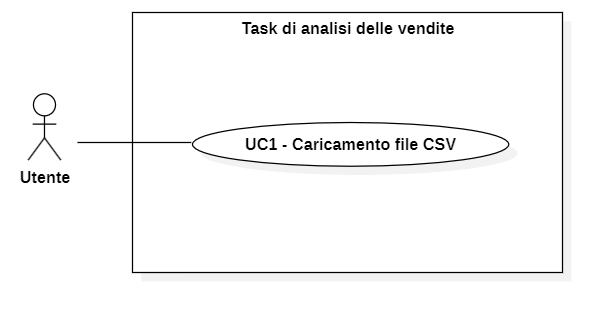
\includegraphics[width=0.9\columnwidth]{usecase/UC1 - Caricamento file CSV.png}
    \caption{UC1 - Caricamento file CSV}
\end{figure}

\usecaseactors{Utente}
\usecasepre{L'utente ha avviato la task di analisi delle vendite}
\usecasedesc{L'utente carica un file CSV contenente i dati delle vendite}
\usecasepost{Il sistema ha caricato il file CSV e lo ha memorizzato in un bucket del Google Cloud Storage}
\label{uc:caricamento-file-csv}
\end{usecase}


\hypertarget{UC2}{}
\begin{usecase}{2}{Selezione lingua per il report}

\begin{figure}[!h] 
    \centering 
    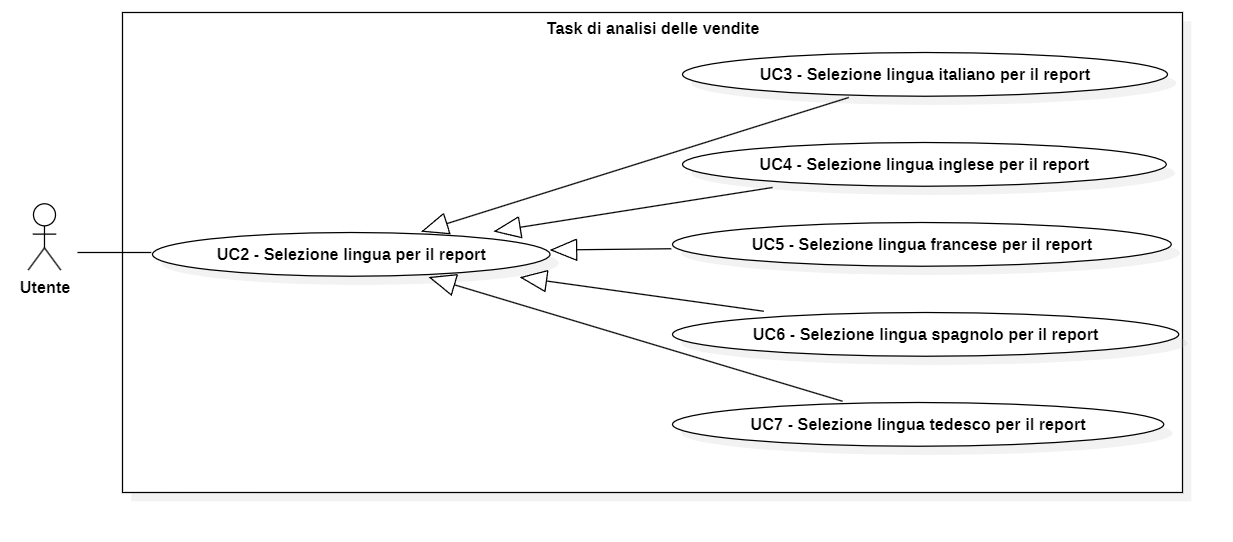
\includegraphics[width=0.9\columnwidth]{usecase/UC2 - Selezione lingua per il report.png}
    \caption{UC2 - Selezione lingua per il report}
\end{figure}

\usecaseactors{Utente}
\usecasepre{L'utente ha avviato la task di analisi delle vendite}
\usecasedesc{L'utente seleziona la lingua in cui desidera generare il report}
\usecasepost{Il sistema ha memorizzato la lingua selezionata}
\usespecial{UC3, UC4, UC5, UC6, UC7}
\label{uc:selezione-lingua-report}
\end{usecase}


\hypertarget{UC3}{}
\begin{usecase}{3}{Selezione lingua italiano per il report}

\usecaseactors{Utente}
\usecasepre{L'utente ha avviato la task di analisi delle vendite}
\usecasedesc{L'utente seleziona la lingua italiano perchè desidera generare il report in italiano}
\usecasepost{Il sistema ha memorizzato la lingua italiano selezionata}
\label{uc:selezione-lingua-italiano-report}
\end{usecase}


\hypertarget{UC4}{}
\begin{usecase}{4}{Selezione lingua inglese per il report}

\usecaseactors{Utente}
\usecasepre{L'utente ha avviato la task di analisi delle vendite}
\usecasedesc{L'utente seleziona la lingua inglese perchè desidera generare il report in inglese}
\usecasepost{Il sistema ha memorizzato la lingua inglese selezionata}
\label{uc:selezione-lingua-inglese-report}
\end{usecase}


\hypertarget{UC5}{}
\begin{usecase}{5}{Selezione lingua francese per il report}

\usecaseactors{Utente}
\usecasepre{L'utente ha avviato la task di analisi delle vendite}
\usecasedesc{L'utente seleziona la lingua francese perchè desidera generare il report in francese}
\usecasepost{Il sistema ha memorizzato la lingua francese selezionata}
\label{uc:selezione-lingua-francese-report}
\end{usecase}


\hypertarget{UC6}{}
\begin{usecase}{6}{Selezione lingua spagnolo per il report}

\usecaseactors{Utente}
\usecasepre{L'utente ha avviato la task di analisi delle vendite}
\usecasedesc{L'utente seleziona la lingua spagnolo perchè desidera generare il report in spagnolo}
\usecasepost{Il sistema ha memorizzato la lingua spagnolo selezionata}
\label{uc:selezione-lingua-spagnolo-report}
\end{usecase}


\hypertarget{UC7}{}
\begin{usecase}{7}{Selezione lingua tedesco per il report}

\usecaseactors{Utente}
\usecasepre{L'utente ha avviato la task di analisi delle vendite}
\usecasedesc{L'utente seleziona la lingua tedesco perchè desidera generare il report in tedesco}
\usecasepost{Il sistema ha memorizzato la lingua tedesco selezionata}
\label{uc:selezione-lingua-tedesco-report}
\end{usecase}


\hypertarget{UC8}{}
\begin{usecase}{8}{Selezione valuta per il report}

\begin{figure}[!h] 
    \centering 
    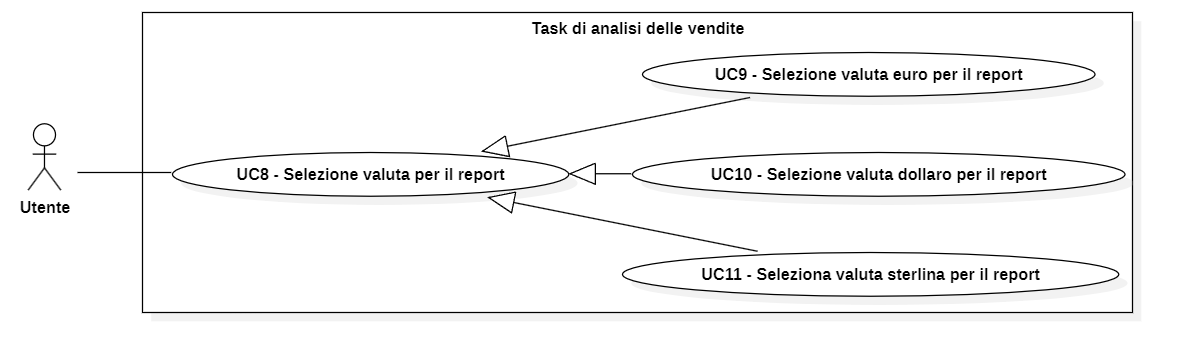
\includegraphics[width=0.9\columnwidth]{usecase/UC8 - Selezione valuta per il report.png}
    \caption{UC8 - Selezione valuta per il report}
\end{figure}

\usecaseactors{Utente}
\usecasepre{L'utente ha avviato la task di analisi delle vendite}
\usecasedesc{L'utente seleziona la valuta in cui desidera generare il report}
\usecasepost{Il sistema ha memorizzato la valuta selezionata}
\usespecial{UC9, UC10, UC11}
\label{uc:selezione-valuta-report}
\end{usecase}


\hypertarget{UC9}{}
\begin{usecase}{9}{Selezione valuta euro per il report}

\usecaseactors{Utente}
\usecasepre{L'utente ha avviato la task di analisi delle vendite}
\usecasedesc{L'utente seleziona la valuta euro perchè desidera generare il report con i valori monetari espressi in euro}
\usecasepost{Il sistema ha memorizzato la valuta euro selezionata}
\label{uc:selezione-valuta-euro-report}
\end{usecase}


\hypertarget{UC10}{}
\begin{usecase}{10}{Selezione valuta dollaro per il report}

\usecaseactors{Utente}
\usecasepre{L'utente ha avviato la task di analisi delle vendite}
\usecasedesc{L'utente seleziona la valuta dollaro perchè desidera generare il report con i valori monetari espressi in dollari}
\usecasepost{Il sistema ha memorizzato la valuta dollaro selezionata}
\label{uc:selezione-valuta-dollaro-report}
\end{usecase}


\hypertarget{UC11}{}
\begin{usecase}{11}{Selezione valuta sterlina per il report}

\usecaseactors{Utente}
\usecasepre{L'utente ha avviato la task di analisi delle vendite}
\usecasedesc{L'utente seleziona la valuta sterlina perchè desidera generare il report con i valori monetari espressi in sterline}
\usecasepost{Il sistema ha memorizzato la valuta sterlina selezionata}
\label{uc:selezione-valuta-sterlina-report}
\end{usecase}


\hypertarget{UC12}{}
\begin{usecase}{12}{Inserimento indirizzo email a cui inviare il report}

\begin{figure}[!h]
    \centering 
    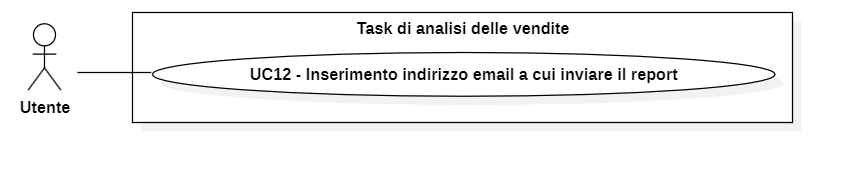
\includegraphics[width=0.9\columnwidth]{usecase/UC12 - Inserimento indirizzo email a cui inviare il report.png}
    \caption{UC12 - Inserimento indirizzo email a cui inviare il report}
\end{figure}

\usecaseactors{Utente}
\usecasepre{L'utente ha avviato la task di analisi delle vendite}
\usecasedesc{L'utente inserisce l'indirizzo email a cui desidera che venga inviato il report generato}
\usecasepost{Il sistema ha memorizzato l'indirizzo email inserito}

\end{usecase}


\hypertarget{UC13}{}
\begin{usecase}{13}{Visualizzazione esito positivo della task}

\begin{figure}[!h]
    \centering 
    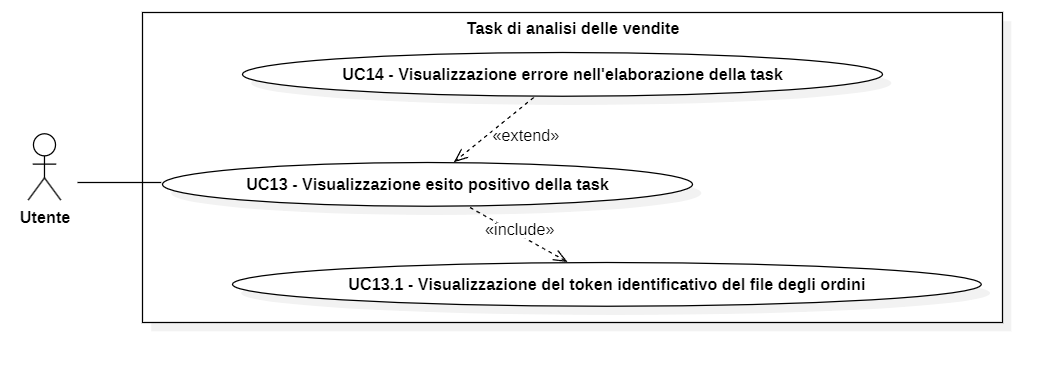
\includegraphics[width=0.9\columnwidth]{usecase/UC13 - Visualizzazione esito positivo della task.png}
    \caption{UC13 - Visualizzazione esito positivo della task}
\end{figure}

\usecaseactors{Utente}
\usecasepre{L'utente ha cliccato sul pulsante di esecuzione della task di analisi delle vendite}
\usecasedesc{L'utente visualizza l'esito positivo della task di analisi delle vendite}
\usecasepost{L'utente ha visualizzato l'esito positivo della task di analisi delle vendite}
\usecasealt{UC14}
\label{uc:visualizzazione-esito-positivo-task}
\end{usecase}


\hypertarget{UC13.1}{}
\begin{usecase}{13.1}{Visualizzazione del token identificativo del file degli ordini}

\usecaseactors{Utente}
\usecasepre{L'utente ha cliccato sul pulsante di esecuzione della task di analisi delle vendite}
\usecasedesc{L'utente visualizza il token identificativo del file degli ordini caricato}
\usecasepost{L'utente ha visualizzato il token identificativo del file degli ordini caricato}
\label{uc:visualizzazione-token-file-ordini}
\end{usecase}


\hypertarget{UC14}{}
\begin{usecase}{14}{Visualizzazione errore nell'elaborazione della task}

\usecaseactors{Utente}
\usecasepre{L'utente ha cliccato sul pulsante di esecuzione della task di analisi delle vendite}
\usecasedesc{L'utente visualizza un errore nell'elaborazione della task di analisi delle vendite}
\usecasepost{L'utente ha visualizzato un errore nell'elaborazione della task di analisi delle vendite}
\label{uc:visualizzazione-errore-task}
\end{usecase}


\hypertarget{UC15}{}
\begin{usecase}{15}{Download report delle vendite}

\begin{figure}[!h] 
    \centering 
    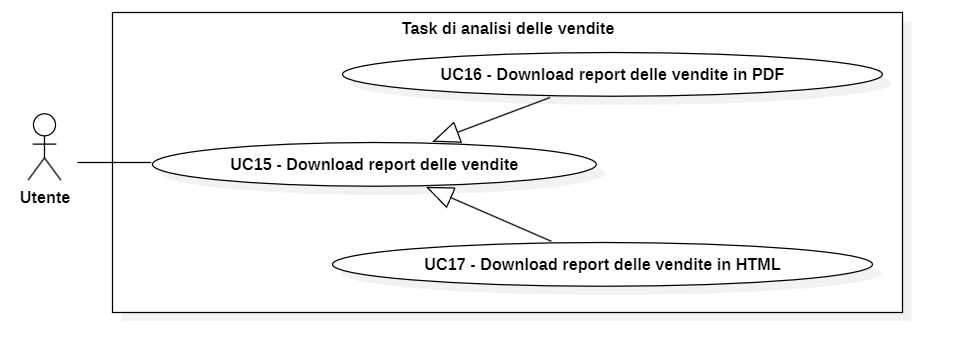
\includegraphics[width=0.9\columnwidth]{usecase/UC15 - Download report delle vendite.png}
    \caption{UC15 - Download report delle vendite}
\end{figure}

\usecaseactors{Utente}
\usecasepre{L'utente ha cliccato sul pulsante di esecuzione della task di analisi delle vendite}
\usecasedesc{L'utente scarica il report delle vendite generato dalla task di analisi delle vendite}
\usecasepost{L'utente ha scaricato il report delle vendite generato dalla task di analisi delle vendite}
\usespecial{UC16, UC17}
\label{uc:download-report-vendite}
\end{usecase}


\hypertarget{UC16}{}
\begin{usecase}{16}{Download report delle vendite in PDF}

\usecaseactors{Utente}
\usecasepre{L'utente ha cliccato sul pulsante di esecuzione della task di analisi delle vendite}
\usecasedesc{L'utente scarica il report delle vendite generato dalla task di analisi delle vendite in formato PDF}
\usecasepost{L'utente ha scaricato il report delle vendite generato dalla task di analisi delle vendite in formato PDF}
\label{uc:download-report-vendite-pdf}
\end{usecase}


\hypertarget{UC17}{}
\begin{usecase}{17}{Download report delle vendite in HTML}

\usecaseactors{Utente}
\usecasepre{L'utente ha cliccato sul pulsante di esecuzione della task di analisi delle vendite}
\usecasedesc{L'utente scarica il report delle vendite generato dalla task di analisi delle vendite in formato HTML}
\usecasepost{L'utente ha scaricato il report delle vendite generato dalla task di analisi delle vendite in formato HTML}
\label{uc:download-report-vendite-html}
\end{usecase}


\hypertarget{UC18}{}
\begin{usecase}{18}{Visualizzazione di un'email contenente il report delle vendite}

\begin{figure}[!h] 
    \centering 
    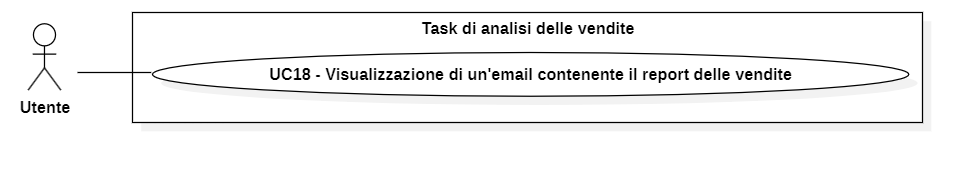
\includegraphics[width=0.9\columnwidth]{usecase/UC18 - Visualizzazione di un'email contenente il report delle vendite.png}
    \caption{UC18 - Visualizzazione di un'email contenente il report delle vendite}
\end{figure}

\usecaseactors{Utente}
\usecasepre{L'utente ha cliccato sul pulsante di esecuzione della task di analisi delle vendite, e poi ha visitato la propria casella di posta elettronica e cliccato sull'email ricevuta contenente il report delle vendite}
\usecasedesc{L'utente visualizza un'email contenente il report delle vendite generato dalla task di analisi delle vendite}
\usecasepost{L'utente ha visualizzato un'email contenente il report delle vendite generato dalla task di analisi delle vendite}
\useinclu{UC18.1, UC18.2, UC18.3}
\label{uc:visualizzazione-email-report-vendite}
\end{usecase}


\hypertarget{UC18.1}{}
\begin{usecase}{18.1}{Visualizzazione dati numerici}

\begin{figure}[!h] 
    \centering 
    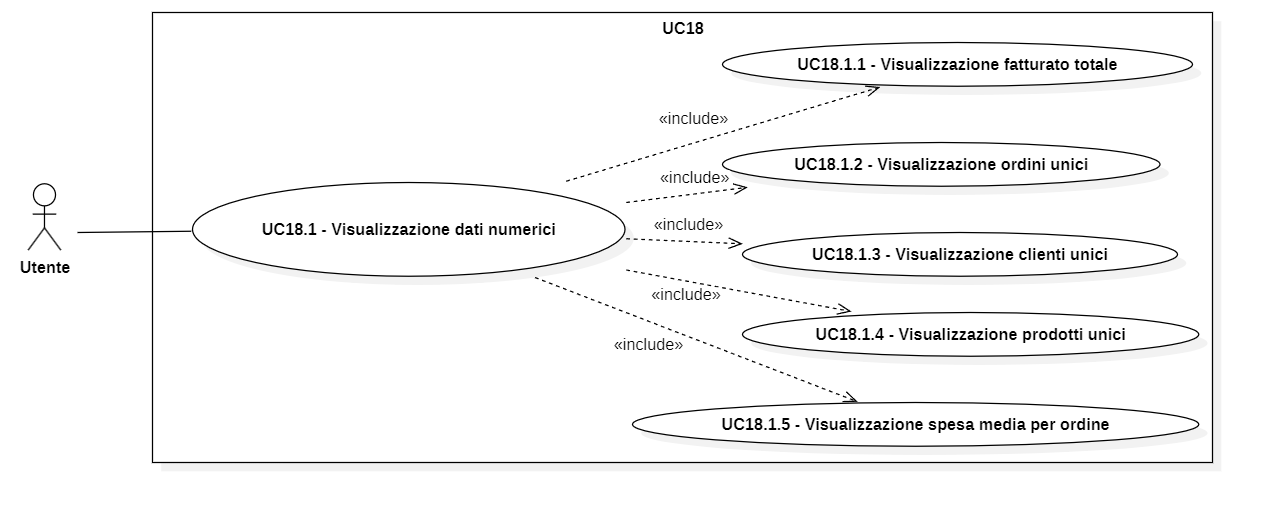
\includegraphics[width=0.9\columnwidth]{usecase/UC18.1 - Visualizzazione dati numerici.png}
    \caption{UC18.1 - Visualizzazione dati numerici}
\end{figure}

\usecaseactors{Utente}
\usecasepre{L'utente ha cliccato sul pulsante di esecuzione della task di analisi delle vendite, e poi ha visitato la propria casella di posta elettronica e cliccato sull'email ricevuta contenente il report delle vendite}
\usecasedesc{L'utente visualizza i dati numerici contenuti nel report delle vendite generato dalla task di analisi delle vendite}
\usecasepost{L'utente ha visualizzato i dati numerici contenuti nel report delle vendite generato dalla task di analisi delle vendite}
\useinclu{18.1.1, 18.1.2, 18.1.3, 18.1.4, 18.1.5}
\label{uc:visualizzazione-dati-numerici}
\end{usecase}


\hypertarget{UC18.1.1}{}
\begin{usecase}{18.1.1}{Visualizzazione fatturato totale}

\usecaseactors{Utente}
\usecasepre{L'utente ha cliccato sul pulsante di esecuzione della task di analisi delle vendite, e poi ha visitato la propria casella di posta elettronica e cliccato sull'email ricevuta contenente il report delle vendite}
\usecasedesc{L'utente visualizza il fatturato totale contenuto nel report delle vendite generato dalla task di analisi delle vendite}
\usecasepost{L'utente ha visualizzato il fatturato totale contenuto nel report delle vendite generato dalla task di analisi delle vendite}
\label{uc:visualizzazione-fatturato-totale}
\end{usecase}


\hypertarget{UC18.1.2}{}
\begin{usecase}{18.1.2}{Visualizzazione ordini unici}

\usecaseactors{Utente}
\usecasepre{L'utente ha cliccato sul pulsante di esecuzione della task di analisi delle vendite, e poi ha visitato la propria casella di posta elettronica e cliccato sull'email ricevuta contenente il report delle vendite}
\usecasedesc{L'utente visualizza il numero di ordini unici contenuti nel report delle vendite generato dalla task di analisi delle vendite}
\usecasepost{L'utente ha visualizzato il numero di ordini unici contenuti nel report delle vendite generato dalla task di analisi delle vendite}
\label{uc:visualizzazione-ordini-unici}
\end{usecase}


\hypertarget{UC18.1.3}{}
\begin{usecase}{18.1.3}{Visualizzazione clienti unici}

\usecaseactors{Utente}
\usecasepre{L'utente ha cliccato sul pulsante di esecuzione della task di analisi delle vendite, e poi ha visitato la propria casella di posta elettronica e cliccato sull'email ricevuta contenente il report delle vendite}
\usecasedesc{L'utente visualizza il numero di clienti unici contenuti nel report delle vendite generato dalla task di analisi delle vendite}
\usecasepost{L'utente ha visualizzato il numero di clienti unici contenuti nel report delle vendite generato dalla task di analisi delle vendite}
\label{uc:visualizzazione-clienti-unici}
\end{usecase}


\hypertarget{UC18.1.4}{}
\begin{usecase}{18.1.4}{Visualizzazione prodotti unici}

\usecaseactors{Utente}
\usecasepre{L'utente ha cliccato sul pulsante di esecuzione della task di analisi delle vendite, e poi ha visitato la propria casella di posta elettronica e cliccato sull'email ricevuta contenente il report delle vendite}
\usecasedesc{L'utente visualizza il numero di prodotti unici contenuti nel report delle vendite generato dalla task di analisi delle vendite}
\usecasepost{L'utente ha visualizzato il numero di prodotti unici contenuti nel report delle vendite generato dalla task di analisi delle vendite}
\label{uc:visualizzazione-prodotti-unici}
\end{usecase}


\hypertarget{UC18.1.5}{}
\begin{usecase}{18.1.5}{Visualizzazione spesa media per ordine}

\usecaseactors{Utente}
\usecasepre{L'utente ha cliccato sul pulsante di esecuzione della task di analisi delle vendite, e poi ha visitato la propria casella di posta elettronica e cliccato sull'email ricevuta contenente il report delle vendite}
\usecasedesc{L'utente visualizza la spesa media per ordine contenuta nel report delle vendite generato dalla task di analisi delle vendite}
\usecasepost{L'utente ha visualizzato la spesa media per ordine contenuta nel report delle vendite generato dalla task di analisi delle vendite}
\label{uc:visualizzazione-spesa-media-per-ordine}
\end{usecase}


\hypertarget{UC18.2}{}
\begin{usecase}{18.2}{Visualizzazione lista di grafici}

\begin{figure}[!h] 
    \centering 
    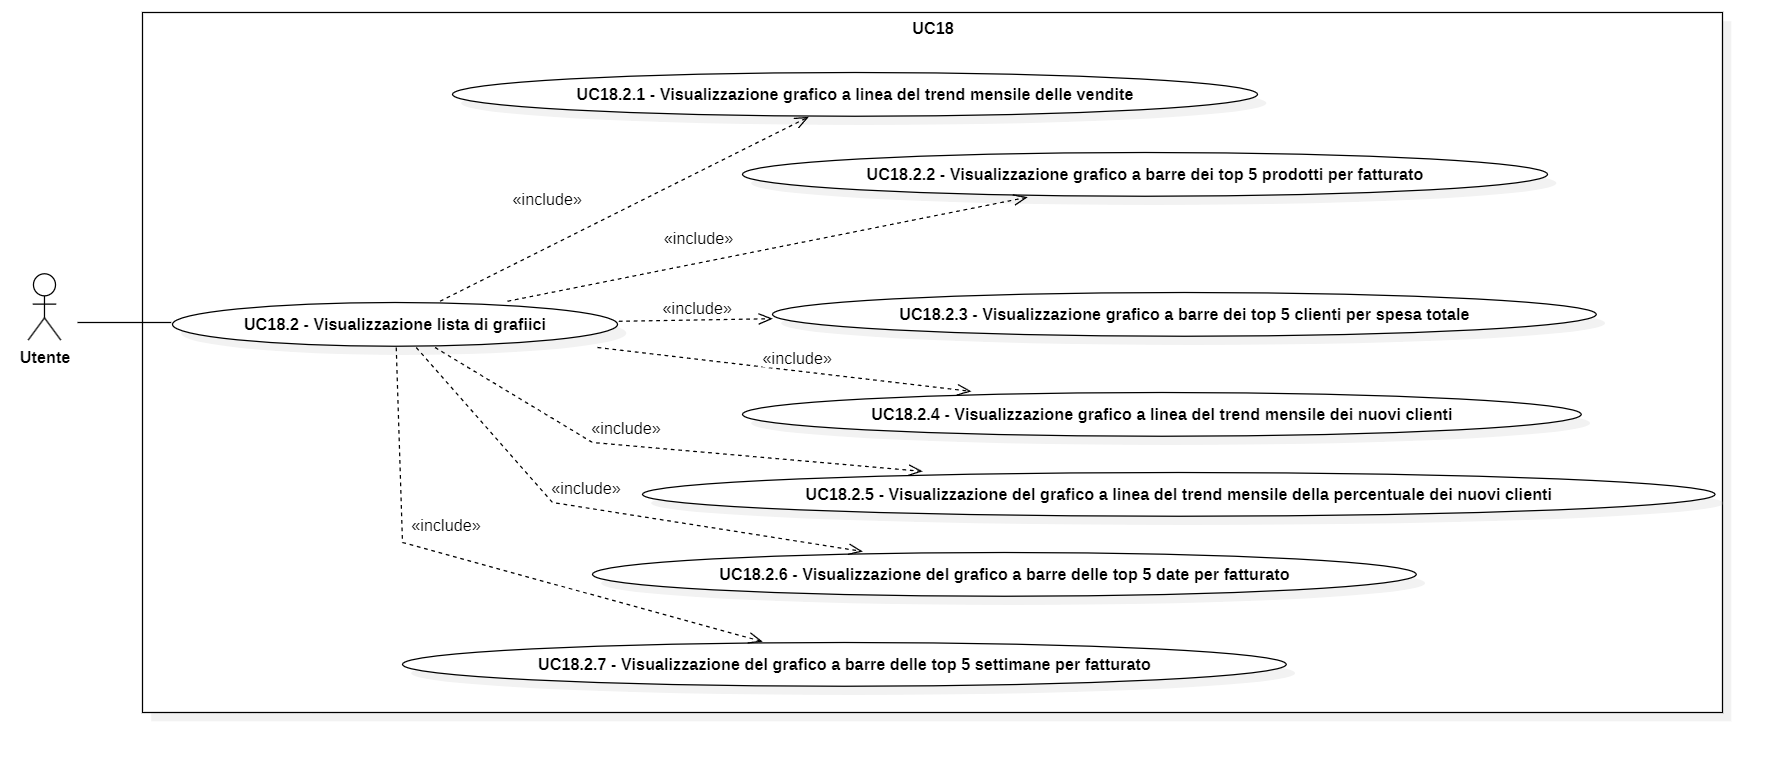
\includegraphics[width=0.9\columnwidth]{usecase/UC18.2 - Visualizzazione lista di grafici.png}
    \caption{UC18.2 - Visualizzazione lista di grafici}
\end{figure}

\usecaseactors{Utente}
\usecasepre{L'utente ha cliccato sul pulsante di esecuzione della task di analisi delle vendite, e poi ha visitato la propria casella di posta elettronica e cliccato sull'email ricevuta contenente il report delle vendite}
\usecasedesc{L'utente visualizza la lista di grafici contenuti nel report delle vendite generato dalla task di analisi delle vendite}
\usecasepost{L'utente ha visualizzato la lista di grafici contenuti nel report delle vendite generato dalla task di analisi delle vendite}
\useinclu{18.2.1, 18.2.2, 18.2.3, 18.2.4, 18.2.5, 18.2.6, 18.2.7}
\label{uc:visualizzazione-lista-grafici}
\end{usecase}


\hypertarget{UC18.2.1}{}
\begin{usecase}{18.2.1}{Visualizzazione grafico a linea del trend mensile delle vendite}

\usecaseactors{Utente}
\usecasepre{L'utente ha cliccato sul pulsante di esecuzione della task di analisi delle vendite, e poi ha visitato la propria casella di posta elettronica e cliccato sull'email ricevuta contenente il report delle vendite}
\usecasedesc{L'utente visualizza il grafico a linea del trend mensile delle vendite contenuto nel report delle vendite generato dalla task di analisi delle vendite}
\usecasepost{L'utente ha visualizzato il grafico a linea del trend mensile delle vendite contenuto nel report delle vendite generato dalla task di analisi delle vendite}
\label{uc:visualizzazione-grafico-trend-mensile-vendite}
\end{usecase}


\hypertarget{UC18.2.2}{}
\begin{usecase}{18.2.2}{Visualizzazione grafico a barre dei top 5 prodotti per fatturato}

\usecaseactors{Utente}
\usecasepre{L'utente ha cliccato sul pulsante di esecuzione della task di analisi delle vendite, e poi ha visitato la propria casella di posta elettronica e cliccato sull'email ricevuta contenente il report delle vendite}
\usecasedesc{L'utente visualizza il grafico a barre dei top 5 prodotti per fatturato contenuto nel report delle vendite generato dalla task di analisi delle vendite}
\usecasepost{L'utente ha visualizzato il grafico a barre dei top 5 prodotti per fatturato contenuto nel report delle vendite generato dalla task di analisi delle vendite}
\label{uc:visualizzazione-grafico-top-5-prodotti-fatturato}
\end{usecase}


\hypertarget{UC18.2.3}{}
\begin{usecase}{18.2.3}{Visualizzazione grafico a barre dei top 5 clienti per spesa totale}

\usecaseactors{Utente}
\usecasepre{L'utente ha cliccato sul pulsante di esecuzione della task di analisi delle vendite, e poi ha visitato la propria casella di posta elettronica e cliccato sull'email ricevuta contenente il report delle vendite}
\usecasedesc{L'utente visualizza il grafico a barre dei top 5 clienti per spesa totale contenuto nel report delle vendite generato dalla task di analisi delle vendite}
\usecasepost{L'utente ha visualizzato il grafico a barre dei top 5 clienti per spesa totale contenuto nel report delle vendite generato dalla task di analisi delle vendite}
\label{uc:visualizzazione-grafico-top-5-clienti-spesa-totale}
\end{usecase}


\hypertarget{UC18.2.4}{}
\begin{usecase}{18.2.4}{Visualizzazione grafico a linea del trend mensile dei nuovi clienti}

\usecaseactors{Utente}
\usecasepre{L'utente ha cliccato sul pulsante di esecuzione della task di analisi delle vendite, e poi ha visitato la propria casella di posta elettronica e cliccato sull'email ricevuta contenente il report delle vendite}
\usecasedesc{L'utente visualizza il grafico a linea del trend mensile dei nuovi clienti contenuto nel report delle vendite generato dalla task di analisi delle vendite}
\usecasepost{L'utente ha visualizzato il grafico a linea del trend mensile dei nuovi clienti contenuto nel report delle vendite generato dalla task di analisi delle vendite}
\label{uc:visualizzazione-grafico-trend-mensile-nuovi-clienti}
\end{usecase}


\hypertarget{UC18.2.5}{}
\begin{usecase}{18.2.5}{Visualizzazione del grafico a linea del trend mensile della percentuale dei nuovi clienti}

\usecaseactors{Utente}
\usecasepre{L'utente ha cliccato sul pulsante di esecuzione della task di analisi delle vendite, e poi ha visitato la propria casella di posta elettronica e cliccato sull'email ricevuta contenente il report delle vendite}
\usecasedesc{L'utente visualizza il grafico a linea del trend mensile della percentuale dei nuovi clienti contenuto nel report delle vendite generato dalla task di analisi delle vendite}
\usecasepost{L'utente ha visualizzato il grafico a linea del trend mensile della percentuale dei nuovi clienti contenuto nel report delle vendite generato dalla task di analisi delle vendite}
\label{uc:visualizzazione-grafico-trend-mensile-percentuale-nuovi-clienti}
\end{usecase}


\hypertarget{UC18.2.6}{}
\begin{usecase}{18.2.6}{Visualizzazione del grafico a barre delle top 5 date per fatturato}

\usecaseactors{Utente}
\usecasepre{L'utente ha cliccato sul pulsante di esecuzione della task di analisi delle vendite, e poi ha visitato la propria casella di posta elettronica e cliccato sull'email ricevuta contenente il report delle vendite}
\usecasedesc{L'utente visualizza il grafico a barre delle top 5 date per fatturato contenuto nel report delle vendite generato dalla task di analisi delle vendite}
\usecasepost{L'utente ha visualizzato il grafico a barre delle top 5 date per fatturato contenuto nel report delle vendite generato dalla task di analisi delle vendite}
\label{uc:visualizzazione-grafico-top-5-date-fatturato}
\end{usecase}


\hypertarget{UC18.2.7}{}
\begin{usecase}{18.2.7}{Visualizzazione del grafico a barre delle top 5 settimane per fatturato}

\usecaseactors{Utente}
\usecasepre{L'utente ha cliccato sul pulsante di esecuzione della task di analisi delle vendite, e poi ha visitato la propria casella di posta elettronica e cliccato sull'email ricevuta contenente il report delle vendite}
\usecasedesc{L'utente visualizza il grafico a barre delle top 5 settimane per fatturato contenuto nel report delle vendite generato dalla task di analisi delle vendite}
\usecasepost{L'utente ha visualizzato il grafico a barre delle top 5 settimane per fatturato contenuto nel report delle vendite generato dalla task di analisi delle vendite}
\label{uc:visualizzazione-grafico-top-5-settimane-fatturato}
\end{usecase}


\hypertarget{UC18.3}{}
\begin{usecase}{18.3}{Visualizzazione resoconto dell'analisi delle vendite}

\begin{figure}[!h] 
    \centering 
    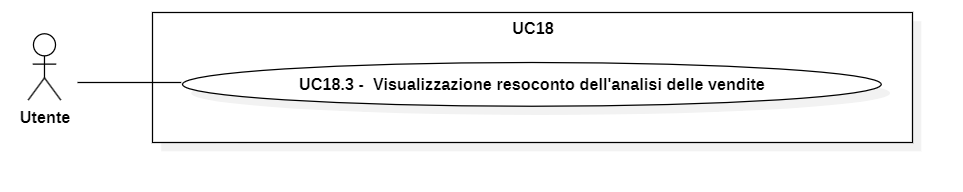
\includegraphics[width=0.9\columnwidth]{usecase/UC18.3 - Visualizzazione resoconto dell'analisi delle vendite.png}
    \caption{UC18.3 - Visualizzazione resoconto dell'analisi delle vendite}
\end{figure}

\usecaseactors{Utente}
\usecasepre{L'utente ha cliccato sul pulsante di esecuzione della task di analisi delle vendite, e poi ha visitato la propria casella di posta elettronica e cliccato sull'email ricevuta contenente il report delle vendite}
\usecasedesc{L'utente visualizza il resoconto dell'analisi delle vendite contenuto nel report delle vendite generato dalla task di analisi delle vendite}
\usecasepost{L'utente ha visualizzato il resoconto dell'analisi delle vendite contenuto nel report delle vendite generato dalla task di analisi delle vendite}
\label{uc:visualizzazione-resoconto-analisi-vendite}
\end{usecase}


\hypertarget{UC18.4}{}
\begin{usecase}{18.4}{Visualizzazione del token identificativo del file degli ordini}

\begin{figure}[!h] 
    \centering 
    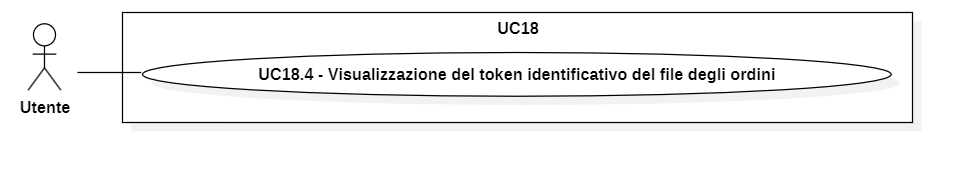
\includegraphics[width=0.9\columnwidth]{usecase/UC18.4 - Visualizzazione del token identificativo del file degli ordini.png}
    \caption{UC18.4 - Visualizzazione del token identificativo del file degli ordini}
\end{figure}

\usecaseactors{Utente}
\usecasepre{L'utente ha cliccato sul pulsante di esecuzione della task di analisi delle vendite, e poi ha visitato la propria casella di posta elettronica e cliccato sull'email ricevuta contenente il report delle vendite}
\usecasedesc{L'utente visualizza il token identificativo del file degli ordini caricato}
\usecasepost{L'utente ha visualizzato il token identificativo del file degli ordini caricato}
\label{uc:visualizzazione-token-file-ordini-mail}
\end{usecase}


\hypertarget{UC19}{}
\begin{usecase}{19}{Inserimento del token identificativo del file degli ordini}

\begin{figure}[!h] 
    \centering 
    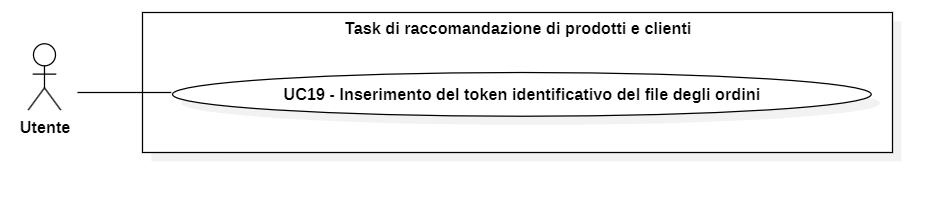
\includegraphics[width=0.9\columnwidth]{usecase/UC19 - Inserimento del token identificativo del file degli ordini.png}
    \caption{UC19 - Inserimento del token identificativo del file degli ordini}
\end{figure}

\usecaseactors{Utente}
\usecasepre{L'utente ha eseguito con successo la task di analisi delle vendite e poi ha avviato la task di raccomandazione di prodotti e clienti}
\usecasedesc{L'utente inserisce il token identificativo del file degli ordini, che era stato generato dalla task di analisi delle vendite}
\usecasepost{Il sistema ricerca il bucket corrispondente al token identificativo all'interno del Google Cloud Storage}
\label{uc:inserimento-nome-file-csv}
\end{usecase}


\hypertarget{UC20}{}
\begin{usecase}{20}{Selezione tipo di raccomandazione}

\begin{figure}[!h] 
    \centering 
    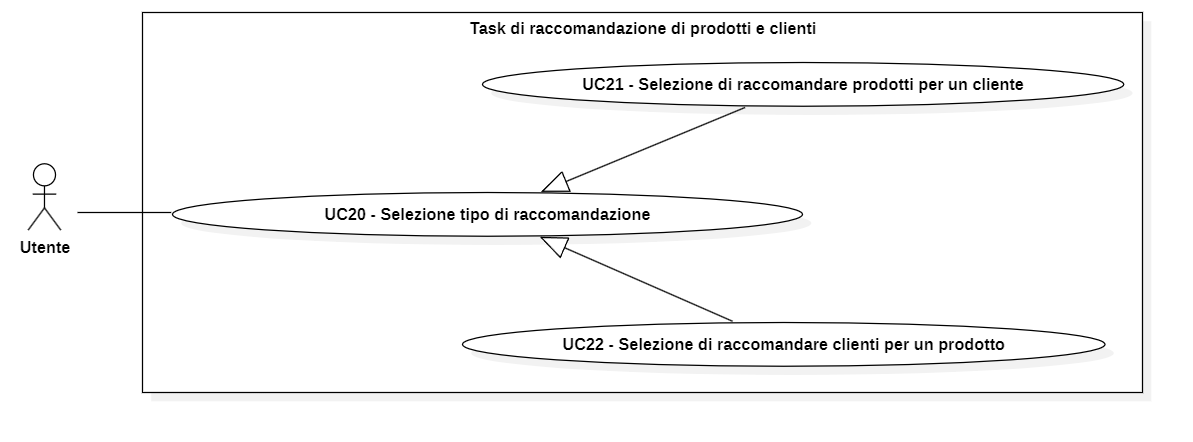
\includegraphics[width=0.9\columnwidth]{usecase/UC20 - Selezione tipo di raccomandazione.png}
    \caption{UC20 - Selezione tipo di raccomandazione}
\end{figure}

\usecaseactors{Utente}
\usecasepre{L'utente ha eseguito con successo la task di analisi delle vendite e poi ha avviato la task di raccomandazione di prodotti e clienti}
\usecasedesc{L'utente seleziona la tipologia di raccomandazione che desidera che venga eseguita, tra le seguenti: "Raccomandare prodotti per un cliente" o "Raccomandare clienti per un prodotto"}
\usecasepost{Il sistema ha memorizzato il tipo di raccomandazione selezionato}
\usespecial{UC21, UC22}
\label{uc:selezione-tipo-elemento}
\end{usecase}


\hypertarget{UC21}{}
\begin{usecase}{21}{Selezione di raccomandare prodotti per un cliente}

\usecaseactors{Utente}
\usecasepre{L'utente ha eseguito con successo la task di analisi delle vendite e poi ha avviato la task di raccomandazione di prodotti e clienti}
\usecasedesc{L'utente seleziona il tipo di raccomandazione "Raccomandare prodotti per un cliente"}
\usecasepost{Il sistema ha memorizzato il tipo di raccomandazione "Raccomandare prodotti per un cliente" selezionato}
\label{uc:selezione-raccomandare-prodotti}
\end{usecase}


\hypertarget{UC22}{}
\begin{usecase}{22}{Selezione di raccomandare clienti per un prodotto}

\usecaseactors{Utente}
\usecasepre{L'utente ha eseguito con successo la task di analisi delle vendite e poi ha avviato la task di raccomandazione di prodotti e clienti}
\usecasedesc{L'utente seleziona il tipo di raccomandazione "Raccomandare clienti per un prodotto"}
\usecasepost{Il sistema ha memorizzato il tipo di raccomandazione "Raccomandare clienti per un prodotto" selezionato}
\label{uc:selezione-raccomandare-clienti}
\end{usecase}


\hypertarget{UC23}{}
\begin{usecase}{23}{Inserimento nome elemento a cui raccomandare}

\begin{figure}[!h] 
    \centering 
    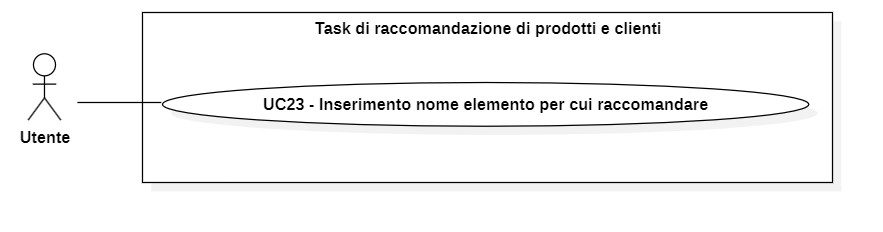
\includegraphics[width=0.9\columnwidth]{usecase/UC23 - Inserimento nome elemento a cui raccomandare.png}
    \caption{UC23 - Inserimento nome elemento a cui raccomandare}
\end{figure}

\usecaseactors{Utente}
\usecasepre{L'utente ha eseguito con successo la task di analisi delle vendite e poi ha avviato la task di raccomandazione di prodotti e clienti}
\usecasedesc{L'utente inserisce il nome dell'elemento a cui desidera che vengano raccomandati prodotti o clienti, a seconda del tipo di raccomandazione selezionato}
\usecasepost{Il sistema cerca l'elemento corrispondente al nome inserito all'interno del file salvato nel Google Cloud Storage}
\label{uc:inserimento-nome-elemento}
\end{usecase}


\hypertarget{UC24}{}
\begin{usecase}{24}{Inserimento del numero di raccomandazioni desiderate}

\begin{figure}[!h] 
    \centering 
    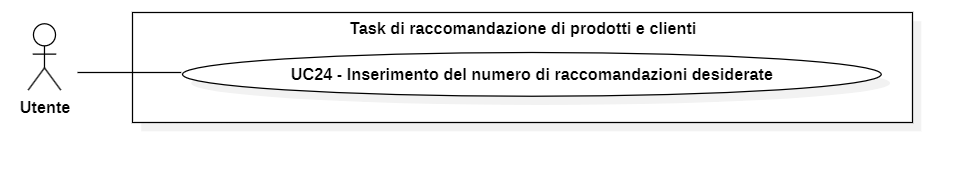
\includegraphics[width=0.9\columnwidth]{usecase/UC24 - Inserimento del numero di raccomandazioni desiderate.png}
    \caption{UC24 - Inserimento del numero di raccomandazioni desiderate}
\end{figure}

\usecaseactors{Utente}
\usecasepre{L'utente ha eseguito con successo la task di analisi delle vendite e poi ha avviato la task di raccomandazione di prodotti e clienti}
\usecasedesc{L'utente inserisce il numero di raccomandazioni che desidera che vengano generate}
\usecasepost{Il sistema ha memorizzato il numero di raccomandazioni desiderate}
\label{uc:inserimento-numero-raccomandazioni}
\end{usecase}


\hypertarget{UC25}{}
\begin{usecase}{25}{Selezione lingua per la raccomandazione}

\begin{figure}[!h] 
    \centering 
    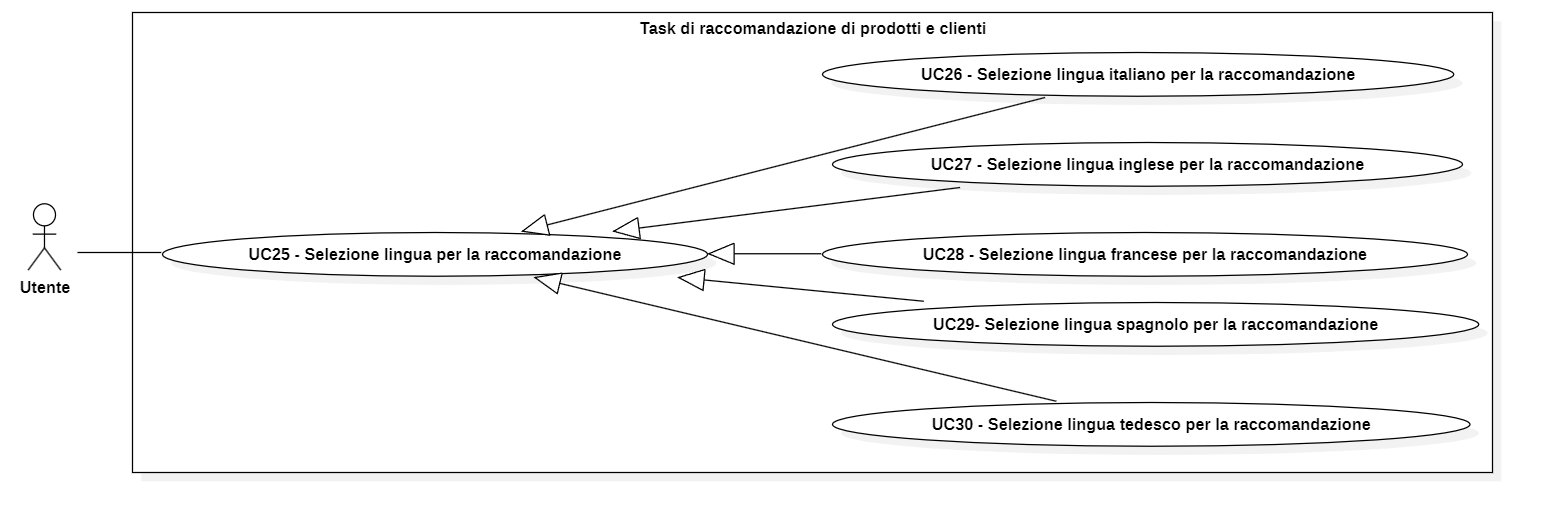
\includegraphics[width=0.9\columnwidth]{usecase/UC25 - Selezione lingua per la raccomandazione.png}
    \caption{UC25 - Selezione lingua per la raccomandazione}
\end{figure}

\usecaseactors{Utente}
\usecasepre{L'utente ha eseguito con successo la task di analisi delle vendite e poi ha avviato la task di raccomandazione di prodotti e clienti}
\usecasedesc{L'utente seleziona la lingua in cui desidera generare la raccomandazione}
\usecasepost{Il sistema ha memorizzato la lingua selezionata}
\usespecial{UC26, UC27, UC28, UC29, UC30}
\label{uc:selezione-lingua-raccomandazione}
\end{usecase}


\hypertarget{UC26}{}
\begin{usecase}{26}{Selezione lingua italiano per la raccomandazione}

\usecaseactors{Utente}
\usecasepre{L'utente ha eseguito con successo la task di analisi delle vendite e poi ha avviato la task di raccomandazione di prodotti e clienti}
\usecasedesc{L'utente seleziona la lingua italiano perchè desidera generare la raccomandazione in italiano}
\usecasepost{Il sistema ha memorizzato la lingua italiano selezionata}
\label{uc:selezione-lingua-italiano-raccomandazione}
\end{usecase}


\hypertarget{UC27}{}
\begin{usecase}{27}{Selezione lingua inglese per la raccomandazione}

\usecaseactors{Utente}
\usecasepre{L'utente ha eseguito con successo la task di analisi delle vendite e poi ha avviato la task di raccomandazione di prodotti e clienti}
\usecasedesc{L'utente seleziona la lingua inglese perchè desidera generare la raccomandazione in inglese}
\usecasepost{Il sistema ha memorizzato la lingua inglese selezionata}
\label{uc:selezione-lingua-inglese-raccomandazione}
\end{usecase}


\hypertarget{UC28}{}
\begin{usecase}{28}{Selezione lingua francese per la raccomandazione}

\usecaseactors{Utente}
\usecasepre{L'utente ha eseguito con successo la task di analisi delle vendite e poi ha avviato la task di raccomandazione di prodotti e clienti}
\usecasedesc{L'utente seleziona la lingua francese perchè desidera generare la raccomandazione in francese}
\usecasepost{Il sistema ha memorizzato la lingua francese selezionata}
\label{uc:selezione-lingua-francese-raccomandazione}
\end{usecase}


\hypertarget{UC29}{}
\begin{usecase}{29}{Selezione lingua spagnolo per la raccomandazione}

\usecaseactors{Utente}
\usecasepre{L'utente ha eseguito con successo la task di analisi delle vendite e poi ha avviato la task di raccomandazione di prodotti e clienti}
\usecasedesc{L'utente seleziona la lingua spagnolo perchè desidera generare la raccomandazione in spagnolo}
\usecasepost{Il sistema ha memorizzato la lingua spagnolo selezionata}
\label{uc:selezione-lingua-spagnolo-raccomandazione}
\end{usecase}


\hypertarget{UC30}{}
\begin{usecase}{30}{Selezione lingua tedesco per la raccomandazione}

\usecaseactors{Utente}
\usecasepre{L'utente ha eseguito con successo la task di analisi delle vendite e poi ha avviato la task di raccomandazione di prodotti e clienti}
\usecasedesc{L'utente seleziona la lingua tedesco perchè desidera generare la raccomandazione in tedesco}
\usecasepost{Il sistema ha memorizzato la lingua tedesco selezionata}
\label{uc:selezione-lingua-tedesco-raccomandazione}
\end{usecase}


\hypertarget{UC31}{}
\begin{usecase}{31}{Visualizzazione classifica elementi raccomandati}

\begin{figure}[!h]
    \centering 
    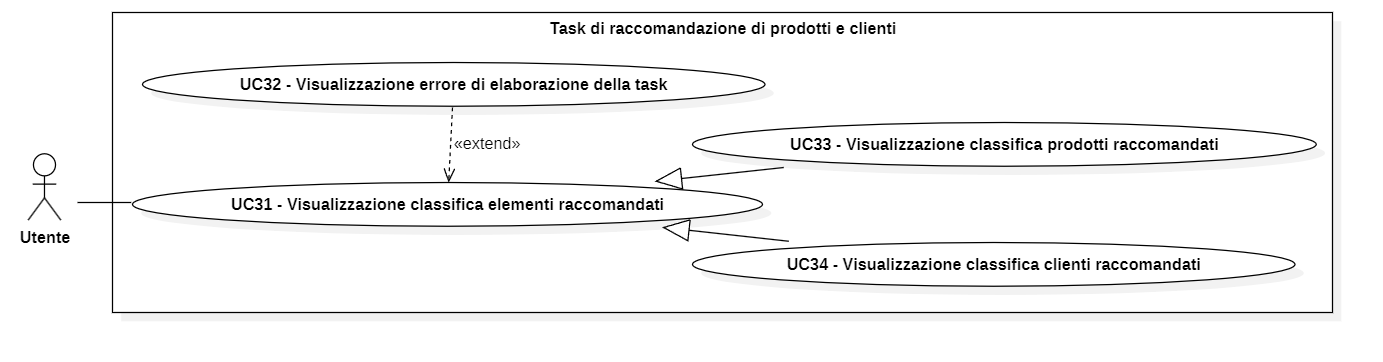
\includegraphics[width=0.9\columnwidth]{usecase/UC31 - Visualizzazione classifica elementi raccomandati.png}
    \caption{UC31 - Visualizzazione classifica elementi raccomandati}
\end{figure}

\usecaseactors{Utente}
\usecasepre{L'utente ha cliccato sul pulsante di esecuzione della task di raccomandazione di prodotti e clienti}
\usecasedesc{L'utente visualizza la classifica degli elementi raccomandati}
\usecasepost{L'utente ha visualizzato la classifica degli elementi raccomandati}
\usecasealt{UC32}
\usespecial{UC33, UC34}
\label{uc:visualizzazione-classifica-elementi-raccomandati}
\end{usecase}


\hypertarget{UC32}{}
\begin{usecase}{32}{Visualizzazione errore di elaborazione della task}

\usecaseactors{Utente}
\usecasepre{L'utente ha cliccato sul pulsante di esecuzione della task di raccomandazione di prodotti e clienti}
\usecasedesc{L'utente visualizza un errore nell'elaborazione della task di raccomandazione di prodotti e clienti}
\usecasepost{L'utente ha visualizzato un errore nell'elaborazione della task di raccomandazione di prodotti e clienti}
\label{uc:visualizzazione-errore-elaborazione-task}
\end{usecase}


\hypertarget{UC33}{}
\begin{usecase}{33}{Visualizzazione classifica prodotti raccomandati}

\usecaseactors{Utente}
\usecasepre{L'utente ha cliccato sul pulsante di esecuzione della task di raccomandazione di prodotti e clienti}
\usecasedesc{L'utente visualizza la classifica dei prodotti raccomandati}
\usecasepost{L'utente ha visualizzato la classifica dei prodotti raccomandati}
\label{uc:visualizzazione-classifica-prodotti-raccomandati}
\end{usecase}


\hypertarget{UC34}{}
\begin{usecase}{34}{Visualizzazione classifica clienti raccomandati}

\usecaseactors{Utente}
\usecasepre{L'utente ha cliccato sul pulsante di esecuzione della task di raccomandazione di prodotti e clienti}
\usecasedesc{L'utente visualizza la classifica dei clienti raccomandati}
\usecasepost{L'utente ha visualizzato la classifica dei clienti raccomandati}
\label{uc:visualizzazione-classifica-clienti-raccomandati}
\end{usecase}



\newpage









\section{Tracciamento dei requisiti}

Da un'attenta analisi dei requisiti e dei casi d'uso effettuata sul progetto è stata stilata la tabella che traccia i requisiti in rapporto ai casi d'uso.

Sono stati individuati diversi tipi di requisiti e si è quindi fatto utilizzo di un codice identificativo per distinguerli.

Il codice dei requisiti è così strutturato:
\begin{center}
    \textbf{R[importanza][tipo]-[numero]}
\end{center}
dove:
\begin{itemize}
	\item L'importanza può essere O per i requisiti obbligatori, D per quelli desiderabili oppure Z per quelli opzionali;
	\item Il tipo può essere F per i requisiti funzionali, Q per quelli qualitativi oppure V per quelli di vincolo;
	\item Il numero è un valore numerico progressivo che identifica univocamente un requisito.
\end{itemize}
Nelle tabelle \ref{tab:requisiti-funzionali}, \ref{tab:requisiti-qualitativi} e \ref{tab:requisiti-vincolo} sono riassunti, rispettivamente, i requisiti funzionali, qualitativi e di vincolo, e l’eventuale loro tracciamento con i casi d'uso delineati in fase di analisi.


\subsection{Requisiti funzionali}

\RequisitiTable
  {Tabella di tracciamento dei requisiti funzionali}
  {tab:requisiti-funzionali}
  {\textbf{Requisito} & \textbf{Descrizione} & \textbf{Fonti}}

ROF-1 & Il sistema deve permettere all'utente di caricare un file CSV contenente gli ordini. & \hyperlink{UC1}{UC1} \\ \hline
ROF-2 & Il sistema deve permettere all'utente di selezionare la lingua da usare per generare il report, tra italiano, inglese, francese, spagnolo e tedesco. & \hyperlink{UC2}{UC2}, \hyperlink{UC3}{UC3}, \hyperlink{UC4}{UC4}, \hyperlink{UC5}{UC5}, \hyperlink{UC6}{UC6} e \hyperlink{UC7}{UC7} \\ \hline
ROF-3 & Il sistema deve permettere all'utente di selezionare la valuta da usare per generare il report, tra euro, dollaro e sterlina. & \hyperlink{UC8}{UC8}, \hyperlink{UC9}{UC9}, \hyperlink{UC10}{UC10} e \hyperlink{UC11}{UC11} \\ \hline
ROF-4 & Il sistema deve permettere all'utente di inserire l'indirizzo email a cui inviare il report generato dalla task di analisi delle vendite. & \hyperlink{UC12}{UC12} \\ \hline
ROF-5 & Nel caso la task di analisi delle vendite sia stata eseguita correttamente, il sistema deve permettere all'utente di visualizzare l'esito positivo della task. & \hyperlink{UC13}{UC13} \\ \hline
ROF-6 & Nel caso la task di analisi delle vendite sia stata eseguita correttamente, il sistema deve permettere all'utente di visualizzare il token identificativo del bucket di Google Cloud Storage in cui è stato salvato il file degli ordini, e di copiarlo negli appunti. & Azienda, \hyperlink{UC13.1}{UC13.1} \\ \hline
ROF-7 & Nel caso avvenga un imprevisto, il sistema deve permettere all'utente di visualizzare un messaggio che segnala un errore di elaborazione della task. & \hyperlink{UC14}{UC14} \\ \hline
ROF-8 & Il sistema deve permettere all'utente di scaricare il report generato dalla task di analisi delle vendite, in formato PDF. & \hyperlink{UC15}{UC15}, \hyperlink{UC16}{UC16}\\ \hline
RDF-9 & Il sistema deve permettere all'utente di scaricare il report generato dalla task di analisi delle vendite, in formato HTML. & \hyperlink{UC15}{UC15}, \hyperlink{UC17}{UC17} \\ \hline
RZF-10 & Il sistema deve inviare il report generato dalla task di analisi delle vendite all'indirizzo email inserito dall'utente. Il testo della mail deve contenere l'HTML del report, e i file PDF e HTML devono essere inviati in allegato. & \hyperlink{UC18}{UC18} \\ \hline
ROF-11 & Nel report delle vendite generato, l'utente deve visualizzare alcuni dati numerici legati alle vendite. & Azienda, \hyperlink{18.1}, \hyperlink{UC18.1.1}{UC18.1.1}, \hyperlink{UC18.1.2}{UC18.1.2}, \hyperlink{UC18.1.3}{UC18.1.3}, \hyperlink{UC18.1.4}{UC18.1.4} e \hyperlink{UC18.1.5}{UC18.1.5} \\ \hline
ROF-12 & Nel report delle vendite generato, l'utente deve visualizzare alcuni grafici generati a partire dai dati delle vendite. & Azienda, \hyperlink{UC18.2}{UC18.2}, \hyperlink{UC18.2.1}{UC18.2.1}, \hyperlink{UC18.2.2}{UC18.2.2}, \hyperlink{UC18.2.3}{UC18.2.3}, \hyperlink{UC18.2.4}{UC18.2.4}, \hyperlink{UC18.2.5}{UC18.2.5}, \hyperlink{UC18.2.6}{UC18.2.6} e \hyperlink{UC18.2.7}{UC18.2.7} \\ \hline
ROF-13 & Nel report delle vendite generato, l'utente deve visualizzare un resoconto dell'analisi delle vendite, generato dall'LLM. & Azienda, \hyperlink{UC18.3}{UC18.3} \\ \hline
RZF-14 & Nella mail inviata all'utente, l'utente deve visualizzare il token identificativo del bucket di Google Cloud Storage in cui è stato salvato il file degli ordini, e deve poterlo copiare negli appunti. & Azienda, \hyperlink{UC18.4}{UC18.4} \\ \hline
ROF-15 & Il sistema deve permettere all'utente di inserire il token identificativo del bucket di Google Cloud Storage in cui è stato salvato il file degli ordini, il quale era stato generato e mostrato nella task di analisi delle vendite. & \hyperlink{UC19}{UC19} \\ \hline
ROF-16 & Il sistema deve permettere all'utente di selezionare il tipo di raccomandazione da svolgere, tra "Raccomandare prodotti per un cliente" e "Raccomandare clienti per un prodotto". & \hyperlink{UC20}{UC20}, \hyperlink{UC21}{UC21} e \hyperlink{UC22}{UC22} \\ \hline
ROF-17 & Il sistema deve permettere all'utente di inserire il nome dell'elemento a cui desidera che vengano raccomandati prodotti o clienti, a seconda del tipo di raccomandazione selezionato. & \hyperlink{UC23}{UC23} \\ \hline
ROF-18 & Il sistema deve permettere all'utente di inserire il numero di raccomandazioni che desidera che vengano generate. & \hyperlink{UC24}{UC24} \\ \hline
ROF-19 & Il sistema deve permettere all'utente di selezionare la lingua da usare per generare la raccomandazione, tra italiano, inglese, francese, spagnolo e tedesco. & \hyperlink{UC25}{UC25}, \hyperlink{UC26}{UC26}, \hyperlink{UC27}{UC27}, \hyperlink{UC28}{UC28}, \hyperlink{UC29}{UC29} e \hyperlink{UC30}{UC30} \\ \hline
ROF-20 & Nel caso la task di raccomandazione sia stata eseguita correttamente, il sistema deve permettere all'utente di visualizzare la classifica degli elementi raccomandati. & \hyperlink{UC31}{UC31}, \hyperlink{UC33}{UC33} e \hyperlink{UC34}{UC34} \\ \hline
ROF-21 & Nel caso avvenga un imprevisto, il sistema deve permettere all'utente di visualizzare un messaggio che segnala un errore di elaborazione della task. & \hyperlink{UC32}{UC32} \\ \hline

\end{longtable}


\subsection{Requisiti qualitativi}

\RequisitiTable
  {Tabella di tracciamento dei requisiti qualitativi}
  {tab:requisiti-qualitativi}
  {\textbf{Requisito} & \textbf{Descrizione} & \textbf{Fonti}}

ROQ-1 & Il lavoro svolto deve essere opportunamente documentato. & OO6 \\ \hline
ROQ-2 & Il codice prodotto deve essere completamente coperto da test di unità. & OO6 \\ \hline
ROQ-3 & Le risposte prodotte dall'LLM devono essere testate, dopo aver definito un opportuno metodo di test. & Azienda, OO6 \\ \hline
RDQ-4 & La task di raccomandazione di prodotti e clienti deve produrre un risultato in tempi ragionevoli. & Azienda, OD1 \\ \hline
RZQ-5 & Le raccomandazioni devono essere "Explainable", in modo che un tecnico aziendale possa comprendere il motivo per cui sono stati raccomandati determinati prodotti o clienti come output ad un utente. & OZ2 \\ \hline

\end{longtable}


\subsection{Requisiti di vincolo}

\RequisitiTable
  {Tabella di tracciamento dei requisiti di vincolo}
  {tab:requisiti-vincolo}
  {\textbf{Requisito} & \textbf{Descrizione} & \textbf{Fonti}}

ROV-1 & Le funzionalità devono essere espresse mediante due task create usando la piattaforma Oribea. & OO3, OO4 \\ \hline
ROV-2 & I due progetti software delle due tasks devono essere inseriti nel campo function della schermata di creazione task della piattaforma Oribea. & Azienda, OO1 \\ \hline
ROV-3 & I due progetti software delle due tasks devono essere caricati come due repository nel profilo GitHub dell'azienda Oribea. & Azienda \\ \hline
ROV-4 & Le due task devono utilizzare, come archiviazione, il profilo Google Cloud dell'azienda Oribea. & Azienda, OO2 \\ \hline
ROV-5 & La task di analisi delle vendite deve permettere il download del report in formato PDF. & Azienda, OZ3 \\ \hline
RDV-6 & La task di analisi delle vendite deve permettere il download del report in formato HTML. & OZ3 \\ \hline
RZV-7 & La task di analisi delle vendite deve permettere l'invio del report via e-mail. & OZ3 \\ \hline

\end{longtable}

    \chapter{Report delle vendite}
\label{cap:report-vendite}

\intro{In questo capitolo, vengono descritte le teorie e le tecniche utilizzate per l'analisi delle vendite, con particolare attenzione allo studio dei dati, delle statistiche utili e dei grafici generati. Viene inoltre discusso il beneficio dell'automazione dell'analisi delle vendite in confronto all'alternativa manuale.}



\section{Benefici dell’automazione dell’analisi delle vendite}

La \gls{busintel}\glsfirstoccur{} è un insieme di tecnologie e pratiche che consentono alle aziende di raccogliere, analizzare e presentare dati per supportare il processo decisionale. L'automazione dell'analisi delle vendite rappresenta un passo avanti significativo rispetto all'analisi manuale, offrendo numerosi vantaggi:
\begin{itemize}
    \item \textbf{Efficienza}: l'automazione consente di elaborare grandi volumi di dati in tempi ridotti, riducendo il tempo necessario per generare report e analisi;
    \item \textbf{Accuratezza}: le operazioni automatizzate riducono il rischio di errori umani, garantendo risultati più precisi e affidabili;
    \item \textbf{Scalabilità}: le soluzioni automatizzate possono gestire facilmente l'aumento dei dati e delle richieste di analisi, adattandosi alle esigenze aziendali in crescita;
    \item \textbf{Accessibilità}: i report automatizzati possono essere facilmente condivisi tra i membri del team e le parti interessate, migliorando la collaborazione e la comunicazione;
    \item \textbf{Personalizzazione}: le soluzioni automatizzate possono essere configurate per generare report specifici in base alle esigenze dell'azienda, consentendo un'analisi mirata.
\end{itemize}

Di conseguenza, compito di questo progetto è stato quello di sviluppare un sistema automatizzato per l'analisi delle vendite, in grado di generare report dettagliati e personalizzati in modo rapido ed efficiente. Questo sistema si basa su un processo di raccolta, elaborazione e visualizzazione dei dati, che consente di ottenere informazioni utili per prendere decisioni strategiche e migliorare le performance aziendali.



\section{Studio delle colonne del dataset}
\label{sec:studio-colonne-dataset}
Per poter analizzare le vendite, è fondamentale comprendere le colonne dei dataset dei quali si dispone. Inizialmente, è stato reso disponibile un unico dataset, che d'ora in poi denominerò \emph{orders-export}, fornito dall'azienda di e-commerce committente, dunque le colonne di questo dataset sono state studiate in dettaglio e prese come riferimento per l'analisi delle vendite e per la selezione dei successivi dataset. Le colonne originali di \emph{orders-export} sono le seguenti:
\begin{itemize}
    \item \textbf{Numero Ordine}: identificativo univoco dell'ordine;
    \item \textbf{Data Ordine}: data dell'ordine, che riporta anche il timestamp esatto;
    \item \textbf{ID Cliente}: identificativo univoco del cliente;
    \item \textbf{Nome Cliente}: nome del cliente;
    \item \textbf{Cognome Cliente}: cognome del cliente;
    \item \textbf{Company}: azienda del cliente, se presente;
    \item \textbf{SKU Prodotto}: codice univoco del prodotto (Stock Keeping Unit);
    \item \textbf{ID Prodotto}: identificativo univoco del prodotto;
    \item \textbf{Descrizione Prodotto}: descrizione del prodotto;
    \item \textbf{Quantità}: quantità di prodotto ordinata;
    \item \textbf{Prezzo Unitario}: prezzo unitario del prodotto;
    \item \textbf{Valore Riga}: importo totale dell'acquisto del prodotto. Ciò si deduce solo dai valori contenuti nella colonna, perchè il nominativo della stessa non è stato attribuito in modo corretto.
\end{itemize}

Dopo un primo sguardo alle colonne, è apparsa chiara la necessità di operare un \gls{preprocessing}\glsfirstoccur{} delle stesse, in modo da poter analizzare le vendite in modo standard ed efficace. Ne è l'esempio la colonna \emph{Valore Riga}, che non fa comprendere il suo contenuto a prima vista, e dunque necessita di un cambio di nominativo.

Dopo aver esaminato le colonne del dataset \emph{orders-export}, è stato sviluppato un sistema di preprocessing, descritto più nel dettaglio a livello implementativo nella sezione \S\ref{sec:preprocessing}. In questa fase, sono state scelte le seguenti colonne per l'analisi delle vendite, e il loro nome è stato tradotto in inglese per uniformità con il resto del progetto:
\begin{itemize}
    \item \textbf{Order ID}: identificativo univoco dell'ordine;
    \item \textbf{Order Timestamp}: data e ora esatta dell'ordine;
    \item \textbf{Customer ID}: identificativo univoco del cliente;
    \item \textbf{Customer Name}: nome e cognome del cliente;
    \item \textbf{Product SKU}: codice univoco del prodotto (Stock Keeping Unit);
    \item \textbf{Product Name}: nome o descrizione del prodotto;
    \item \textbf{Unit Price}: prezzo unitario del prodotto;
    \item \textbf{Quantity}: quantità di prodotto ordinata;
    \item \textbf{Total Price}: importo totale relativo all'acquisto del prodotto.
\end{itemize}

Queste colonne sono state dunque prese come riferimento per cercare ulteriori dataset, che potessero essere utili per l'analisi delle vendite. In particolare, sono stati cercati dataset pubblici nella piattaforma Kaggle che contenessero le stesse colonne o colonne riconducibili a quelle standardizzate di \emph{orders-export}. Sono stati trovati i seguenti dataset, nominati con il nome dell'utente che li ha caricati su Kaggle:
\begin{itemize}
    \item \textbf{Anwer};
    \item \textbf{Cornelius};
    \item \textbf{Dee};
    \item \textbf{Delikkaya};
    \item \textbf{Feroze};
    \item \textbf{Segura};
    \item \textbf{Shaw};
    \item \textbf{Swillm};
    \item \textbf{Vaghasiya}.
\end{itemize}

Ogni dataset è stato dunque trattato per ottenere le stesse colonne standardizzate, in modo da poterle confrontare e analizzare in modo efficace.
Inoltre, sono state successivamente aggiunte le seguenti colonne, ricavate dalla colonna "Order Timestamp", per facilitare alcune operazioni di analisi:
\begin{itemize}
    \item \textbf{Order Day}: giorno dell'ordine (1-31);
    \item \textbf{Order Week}: settimana dell'anno in cui è stato effettuato l'ordine (1-53);
    \item \textbf{Order Month}: mese in cui è stato effettuato l'ordine (1-12);
    \item \textbf{Order Year}: anno in cui è stato effettuato l'ordine (YYYY);
    \item \textbf{ISO Date}: data dell'ordine in formato ISO (YYYY-MM-DD);
    \item \textbf{ISO Month}: mese dell'ordine in formato ISO (YYYY-MM).
\end{itemize}

Fatto ciò, in parallelo con lo studio delle statistiche utili e dei grafici, si è visto necessario introdurre delle ulteriori colonne legate alla data, descrittive invece che numeriche, per allinearsi con il linguaggio naturale del report. Siccome il contenuto di tali colonne dipende dalla lingua del report, la loro creazione è ulteriormente descritta a livello implementativo nella sezione \ref{sec:language-processing}, dedicata alla gestione della lingua. Le colonne aggiuntive sono le seguenti:
\begin{itemize}
    \item \textbf{Date}: data dell'ordine in formato naturale, ad esempio "1 gennaio 2023";
    \item \textbf{Month}: mese dell'ordine in formato naturale, ad esempio "gennaio 2023";
    \item \textbf{Week}: settimana dell'anno in formato naturale, ottenuta unendo assieme le date del lunedì e della domenica di tale settimana, ad esempio "3 febbraio 2025 - 9 febbraio 2025".
\end{itemize}

A questo punto, i dataset preprocessati sono pronti per essere analizzati, e le colonne standardizzate sono pronte per essere utilizzate per ricavare le statistiche utili e i grafici.



\section{Valutazione delle statistiche utili}

Per poter analizzare le vendite, è fondamentale comprendere quali statistiche siano utili per ottenere informazioni significative. L'azienda committente, consapevole di ciò, ha fornito un esempio di report delle vendite, visibile nell'immagine \ref{fig:oribea-report-example}, che è stato utilizzato come base per la valutazione delle statistiche utili.

\begin{figure}[!h]
    \centering
    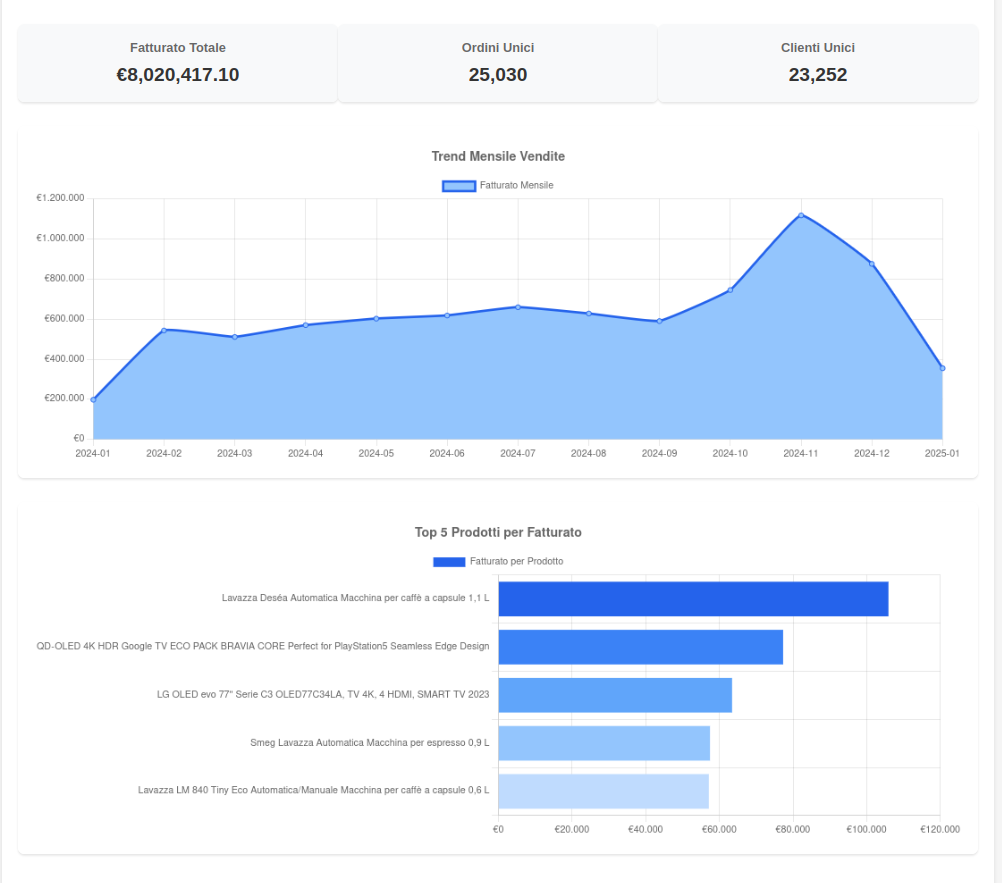
\includegraphics[width=0.9\columnwidth]{Oribea - Esempio di report delle vendite.png}
    \caption{Esempio di report delle vendite fornito da Oribea.}
    \label{fig:oribea-report-example}
\end{figure}

Il report contiene le seguenti statistiche:
\begin{itemize}
    \item \textbf{Fatturato Totale}: il totale delle vendite effettuate nel periodo racchiuso nel dataset;
    \item \textbf{Ordini Unici}: il numero di ordini unici effettuati nel periodo racchiuso nel dataset; questa statistica è necessaria perchè più righe contenenti lo stesso ordine possono essere presenti nel dataset, a causa della possibile presenza di più prodotti nello stesso ordine;
    \item \textbf{Clienti Unici}: il numero di clienti unici che hanno effettuato ordini nel periodo racchiuso nel dataset; questa statistica è necessaria perchè più righe contenenti lo stesso cliente possono essere presenti nel dataset, a causa della possibile presenza di più ordini effettuati dallo stesso cliente.
\end{itemize}

Queste statistiche sono state scelte come base per l'analisi delle vendite, e sono state implementate nel sistema di analisi automatizzato. Successivamente, sono state aggiunte altre statistiche utili, che sono state scelte in base alla loro rilevanza per l'analisi delle vendite e alla loro capacità di fornire informazioni significative. Le statistiche aggiuntive sono le seguenti:
\begin{itemize}
    \item \textbf{Prodotti Unici}: il numero di prodotti unici venduti nel periodo racchiuso nel dataset; questa statistica è necessaria perchè più righe contenenti lo stesso prodotto possono essere presenti nel dataset, a causa della presenza di più ordini effettuati dallo stesso cliente;
    \item \textbf{Spesa Media per Ordine}: la spesa media per ordine, calcolata come il fatturato totale diviso per il numero di ordini unici; questa statistica è utile per comprendere quanto i clienti spendono mediamente per ogni ordine.
\end{itemize}

Successivamente, sono state pensate delle altre elaborazioni statistiche, che però non sono state implementate nel sistema di analisi automatizzato per le ragioni spiegate nelle sezioni \S\ref{sec:recognition-brands} e \S\ref{sec:recognition-categories} legate al \gls{preprocessing}.

A valle di ciò, seppure siano state pensate delle statistiche utili aggiuntive, si è deciso di non implementarle nel sistema di analisi automatizzato. Sono rimaste dunque le cinque statistiche utili descritte in precedenza, che sono state implementate nel sistema di analisi automatizzato e sono state utilizzate per generare il report delle vendite. Queste statistiche sono state scelte in base alla loro rilevanza per l'analisi delle vendite e alla loro capacità di fornire informazioni significative, e sono state ritenute sufficienti per ottenere un'analisi delle vendite efficace e utile.



\section{Valutazione dei grafici utili}

Per poter analizzare le vendite, è fondamentale comprendere quali grafici siano utili per ottenere informazioni significative. Nell'esempio di report delle vendite succitato nell'immagine \ref{fig:oribea-report-example}, sono presenti anche alcuni grafici, che sono stati utilizzati come base per la valutazione dei grafici utili.
I grafici consigliati sono i seguenti:
\begin{itemize}
    \item \textbf{Trend mensile delle vendite}: un grafico a linee che mostra l'andamento delle vendite nel tempo, suddiviso per mese. Questo grafico consente di visualizzare le fluttuazioni delle vendite e di identificare eventuali tendenze stagionali;
    \item \textbf{Top 5 prodotti per fatturato}: un grafico a barre che mostra i cinque prodotti più venduti in termini di fatturato. Questo grafico consente di identificare i prodotti più popolari e redditizi.
\end{itemize}

Il report di esempio ha dunque suggerito l'utilizzo di questi due grafici, che sono stati implementati nel sistema di analisi automatizzato. Non solamente ciò, tale report ha anche suggerito le tipologie di grafici consigliate dall'azienda committente, cioè grafici a linee e a barre, che sono stati quindi scelti per il report per la loro semplicità e chiarezza nella visualizzazione dei dati.

A questo punto, sono stati pensati altri grafici utili, che sono stati implementati nel sistema di analisi automatizzato in parallelo con lo studio del colonne del dataset e del \gls{preprocessing}. I grafici aggiuntivi sono i seguenti:
\begin{itemize}
    \item \textbf{Top 5 clienti per spesa totale}: un grafico a barre che mostra i cinque clienti che hanno speso di più nel periodo racchiuso nel dataset. Questo grafico consente di identificare i clienti più redditizi e di valutare le strategie di fidelizzazione;
    \item \textbf{Trend mensile dei nuovi clienti}: un grafico a linee che mostra l'andamento del numero di nuovi clienti acquisiti nel tempo, suddiviso per mese. Questo grafico consente di valutare l'efficacia delle strategie di marketing e di acquisizione clienti;
    \item \textbf{Trend mennsile della percentuale di nuovi clienti}: un grafico a linee che mostra l'andamento della percentuale di nuovi clienti rispetto al totale dei clienti nel tempo, suddiviso per mese. Questo grafico consente di valutare l'efficacia delle strategie di marketing e di acquisizione clienti in relazione al numero totale di clienti; il valore della percentuale del primo mese è ovviamente 100\%, poiché il numero di nuovi clienti è uguale al numero totale di clienti fino ad allora;
    \item \textbf{Top 5 date per fatturato}: un grafico a barre che mostra le cinque date in cui si è registrato il fatturato più alto. Questo grafico consente di identificare le date più redditizie e di valutare l'efficacia delle strategie di vendita;
    \item \textbf{Top 5 settimane per fatturato}: un grafico a barre che mostra le cinque settimane in cui si è registrato il fatturato più alto. Questo grafico consente di identificare le settimane più redditizie e di valutare l'efficacia delle strategie di vendita.
\end{itemize}

Si nota come sono stati scelti grafici unicamente legati al fatturato, e non a "quantità" o "numero", poiché il fatturato è stata considerata la metrica più importante per l'azienda, cioè quella che fornisce le informazioni più significative. Al contrario, grafici legati a "quantità" o "numero" non sono stati implementati poiché non sono stati ritenuti utili per l'analisi delle vendite.

Molti grafici scelti sono stati legati alla data, poiché si è ritenuto che l'analisi temporale delle vendite fosse fondamentale per comprendere le tendenze e le fluttuazioni delle vendite nel tempo. Da ciò si spiegano le operazioni contemporanee di aggiunta delle colonne legate alla data, descritte sopra nella sezione \S\ref{sec:studio-colonne-dataset}.

Infine, i grafici implementati nel sistema di analisi automatizzato, scelti in base alla loro rilevanza per l'analisi delle vendite e alla loro capacità di fornire informazioni significative, sono stati dunque ritenuti sufficienti per ottenere un'analisi delle vendite efficace e utile.


    \chapter{Sistemi di raccomandazione}
\label{cap:sistemi-raccomandazione}

\intro{Brevissima introduzione al capitolo}\\

\section{Sezione 2}

    \chapter{Progettazione e codifica}
\label{cap:progettazione-codifica}

\intro{Breve introduzione al capitolo}\\

\section{Tecnologie e strumenti}
\label{sec:tecnologie-strumenti}

Di seguito viene data una panoramica delle tecnologie e strumenti utilizzati.

\subsection*{Tecnologia 1}
Descrizione Tecnologia 1.

\subsection*{Tecnologia 2}
Descrizione Tecnologia 2

\section{Ciclo di vita del software}
\label{sec:ciclo-vita-software}

\section{Progettazione}
\label{sec:progettazione}

\subsubsection{Namespace 1} %**************************
Descrizione namespace 1.

\begin{namespacedesc}
    \classdesc{Classe 1}{Descrizione classe 1}
    \classdesc{Classe 2}{Descrizione classe 2}
\end{namespacedesc}


\section{Design Pattern utilizzati}

\section{Codifica}
 % Progettazione e Codifica, non consigliato da Zanella ma lo metto lo stesso
    \chapter{Verifica e validazione}
\label{cap:verifica-validazione}

\intro{Breve introduzione al capitolo}\\

\section{Scelte riguardanti i test}

\section{Test di unità}

\section{Test dell’LLM}
 % Verifica e Validazione, non consigliato da Zanella ma lo metto lo stesso
    \chapter{Conclusioni}
\label{cap:conclusioni}

\intro{In questo capitolo, vengono presentate le conclusioni del progetto, con un riepilogo degli obiettivi raggiunti, delle conoscenze acquisite e dei possibili miglioramenti futuri. Si conclude con una valutazione personale dell'esperienza di sviluppo.}


\section{Considerazioni finali}

Il periodo di tirocinio del laureando Stefani Riccardo ha avuto l'obiettivo di sviluppare un sistema di analisi vendite ed un sistema di raccomandazione per un'azienda di e-commerce, con l'intento di migliorare l'esperienza utente e incrementare le vendite attraverso suggerimenti personalizzati. Il progetto ha richiesto l'analisi dei dati di vendita esistenti, la preparazione dei dati, lo sviluppo di algoritmi di raccomandazione e l'integrazione con l'infrastruttura aziendale. L'implementazione è stata realizzata utilizzando tecnologie moderne come Python, machine learning e integrazione con \gls{googlecloudplatform}.

La maggior parte del tempo è stata dedicata all'analisi e preparazione dei dati di vendita, fase cruciale per garantire l'efficacia del sistema di raccomandazione. Il sistema sviluppato si è rivelato utile per l'azienda, fornendo sia informazioni sui trend di vendita utili per le decisioni strategiche, sia raccomandazioni personalizzate per gli utenti. Questo ha permesso di migliorare l'esperienza di acquisto, aumentando la soddisfazione del cliente e le vendite complessive.

Il sistema è stato implementato in due tasks caricate nella piattaforma Oribea, una per l'analisi delle vendite e l'altra per il sistema di raccomandazione. Sono state inoltre fornite due corrispettive interfacce utente contenenti i form che permettono di accedere alle due funzionalità senza passare attraverso la piattaforma aziendale. Il sistema è stato testato con successo su 10 dataset di vendita reali, dimostrando la sua efficacia e utilità.

È importante sottolineare, tuttavia, che il funzionamento del sistema è strettamente legato alla qualità e completezza del dataset fornito, che infatti deve possedere esattamente le colonne richieste per l'analisi delle vendite e deve possedere un numero sufficiente interazioni cliente-prodotto per generare raccomandazioni significative. Senza le colonne corrette, il sistema restituisce un errore e non può essere utilizzato. Inoltre, se il dataset è troppo scarso, le raccomandazioni generate potrebbero non essere utili o addirittura fuorvianti.


\section{Raggiungimento degli obiettivi}

Tutti i requisiti funzionali e non funzionali identificati nell'analisi iniziale e riportati nel capitolo \S\ref{cap:analisi-requisiti} sono stati raggiunti con successo.

Tra gli obiettivi definiti nel \emph{Piano di Lavoro} e riportati alla sezione \S\ref{sec:obiettivi-stage}, l'unico obiettivo non soddisfatto è stato l'obiettivo opzionale OZ1 relativo all'implementazione di un chatbot che si potesse collegare ad entrambe le \gls{cloudfunctions} e potesse così fornire entrambi i servizi in modo conversazionale, che si è rivelato troppo complesso da realizzare nei tempi disponibili nel tirocinio.


\section{Conoscenze acquisite}

Il tirocinio svolto ha soddisfatto appieno le aspettative: nonostante il progetto sia risultato piuttosto impegnativo, è stato molto utile per approfondire diverse tecnologie ed algoritmi, per acquisire competenze nell’ambito dei sistemi di analisi dati e di raccomandazione e per sperimentare alcune reali applicazioni di strumenti di intelligenza artificiale.

In particolare, le principali nuove conoscenze e competenze maturate durante il
periodo di stage sono le seguenti:

\begin{itemize}
    \item Approfondimento del linguaggio di programmazione Python e delle sue librerie per data science;
    \item Competenze nella preparazione e analisi di grandi volumi di dati;
    \item Competenze nella stesura di analisi delle vendite e reportistica;
    \item Competenze nello sviluppo di sistemi di raccomandazione nell'ambito e-commerce;
    \item Competenze nel collegamento e utilizzo di Google Cloud Platform;
    \item Competenze nell'integrazione con software aziendali pre-esistenti;
    \item Competenze nello sviluppo frontend di interfacce utente;
    \item Competenze di ottimizzazione delle performance di sistemi di analisi dati;
    \item Competenze nella stesura della documentazione tecnica di progetti software.
\end{itemize}


\section{Possibili miglioramenti futuri}

Nonostante il successo generale del sistema sviluppato, alcune funzionalità interessanti non sono state implementate per questioni di tempo e complessità. I possibili miglioramenti futuri includono:

\begin{itemize}
    \item Implementazione di un chatbot che possa interagire con gli utenti e fornire raccomandazioni personalizzate in modo conversazionale, e possa altrettanto comunicare l'analisi delle vendite ai proprietari dell'e-commerce, integrando così le due tasks sviluppate;
    \item Implementazione di un sistema di logging avanzato per monitorare l'esecuzione e le performance delle due tasks;
    \item Implementazione di algoritmi più sofisticati per migliorare la serendipità delle raccomandazioni;
    \item Implementazione di tecniche di \gls{data-reduction} per ridurre la dimensione delle matrici di raccomandazione senza compromettere la qualità dei risultati.
\end{itemize}

\section{Valutazione personale}

Questo progetto di tirocinio ha rappresentato un'importante tappa nel completamento del percorso universitario, permettendo di mettere in pratica le conoscenze teoriche acquisite, in particolare nell'ambito dell'Ingegneria del Software e dell'analisi dati.

L'esperienza è stata particolarmente utile per la crescita professionale a livello tecnico, fornendo competenze pratiche direttamente applicabili nel mondo del lavoro. Tuttavia, lavorando principalmente da remoto e in autonomia, non è stato purtroppo possibile sviluppare competenze di lavoro di squadra o di dinamiche aziendali.

Nonostante questa limitazione, sono complessivamente soddisfatto del risultato finale: gli obiettivi prefissati sono stati raggiunti e le competenze acquisite costituiscono una solida base per il proseguimento degli studi con la laurea magistrale e per future opportunità professionali nel campo dell'informatica e dell'analisi dati.


    \appendix
    \chapter{Appendice A}

\epigraph{Citazione}{Autore della citazione}


    \backmatter
    \printglossary[type=\acronymtype, title=Acronimi e abbreviazioni, toctitle=Acronimi e abbreviazioni]
    \printglossary[type=main, title=Glossario, toctitle=Glossario]

    \cleardoublepage
\chapter{Bibliografia}

\nocite{*}

% Print book bibliography
%\printbibliography[heading=subbibliography,title={Libri},type=book,resetnumbers=true]
\printbibliography[heading=subbibliography,title={Libri},category=libri,resetnumbers=true]

% Print article bibliography
%\printbibliography[heading=subbibliography,title={Riferimenti bibliografici},type=book,resetnumbers=true]
\printbibliography[heading=subbibliography,title={Articoli},category=articoli,resetnumbers=true]

% Print site bibliography
%\printbibliography[heading=subbibliography,title={Siti web consultati},type=online,resetnumbers=true]
\printbibliography[heading=subbibliography,title={Siti web},category=web,resetnumbers=true]

\end{document}
